\chapter{Condiciones de estabilidad}

El capítulo anterior motiva al actual para presentar los resultados de la dinámica que produce la matriz de incidencias $\Lambda$ (Ec. \ref{eqn:MatrizIncidencias}) al integrarse en el sistema de Lotka-Volterra generalizado (ec. \ref{eqn:LK}) y linearizarse produciendo entonces la Matriz de Interacciones (\ref{eqn:MartizInteracciones}). En este capítulo se presentarán los resultados que produce cada etapa del proceso, así como sus características. Nuestra meta es alcanzar los diagramas de transición y compararlos con los resultados de May en sus distintos escenarios; con ello se busca caracterizar estas transiciones y proponer algunos criterios para que se tengan lugar estas transiciones.\\
\\
Para ello se consideraron 3 diferentes simulaciones que comparten algunas similitudes; en concreto la única diferencia es el número de especies o nodos en la red/matriz de incidencias: las simulaciones se consideraron para 25, 50 y 100 especies/nodos, siendo el último caso donde se generó más información. Para poder explorar los resultados de dejaron fijos la mayor cantidad de parámetros para poder observar cambios significativos, de todos los parámetros que hay en la ec. \ref{eqn:LK} únicamente se variaba la forma de la matriz de incidencias $\Lambda$ y que a su vez esta matriz depende de una probabilidad de conectividad $p$ y una fuerza promedio de interacción $\sigma$. En todas las simulaciones la tasa de crecimiento se dejó fija en $r=2$ y la capacidad de carga en $K=5$ para toda especie del sistema. Se integró el sistema con RK4 para un intervalo de tiempo entre 0 y 50 con un paso de integración de $h=0.01$.\\
\\
Además de estos parámetros, siempre se inicializó cada simulación con la condición inicial $\vec{x}_0=\vec{1}$ (dependiendo de la dimensión del sistema) y se consideraron dos escenarios\footnote{solo aplicca para $N=100$}: Matrices de incidencias estructuralmente simétricas y puramente aleatorias, tal y como se visualizó al final del capítulo anterior. En el apéndice (\ref{ch:Ap}), el lector puede darse una idea de como se realizó el proceso de las simulaciones. En cada escenario se presentó cierta cantidad de ruido en las gráficas de estabilidad, por lo que el número de simulaciones fue establecido en función de la disminución de dicho ruido.

\section{Series de tiempo}
Anteriormente se comentaba que las interacciones de la matriz de incidencias $\Lambda$ están volteadas con respecto de la matriz de interacciones $\mathcal{I}$ (ver Definición \ref{def:MatrizInteracciones}), la cooperación en $\mathcal{I}$ se da para las interacciones (++) mientras que para $\Lambda$ se da para $(--)$. Esto es muy importante no perderlo de vista puesto que al tener $N\gg 1$ especies, es difícil poder monitorear el signo de todas las interacciones que intervienen. Si tuviéramos un sistema puramente de competencia, es decir para toda $\alpha_{ij}\in\Lambda$ mayor o igual que cero, entonces no hay forma de que ninguna de las poblaciones participantes sobrepasen la capacidad de carga establecida, tal y como se pudo esbozar en el Ejemplo \ref{eg:2x2}. Por lo tanto obtendríamos series de tiempo caóticas para cada una de las especies por debajo de $K=5$.
\begin{figure}[h!]
	\centering
	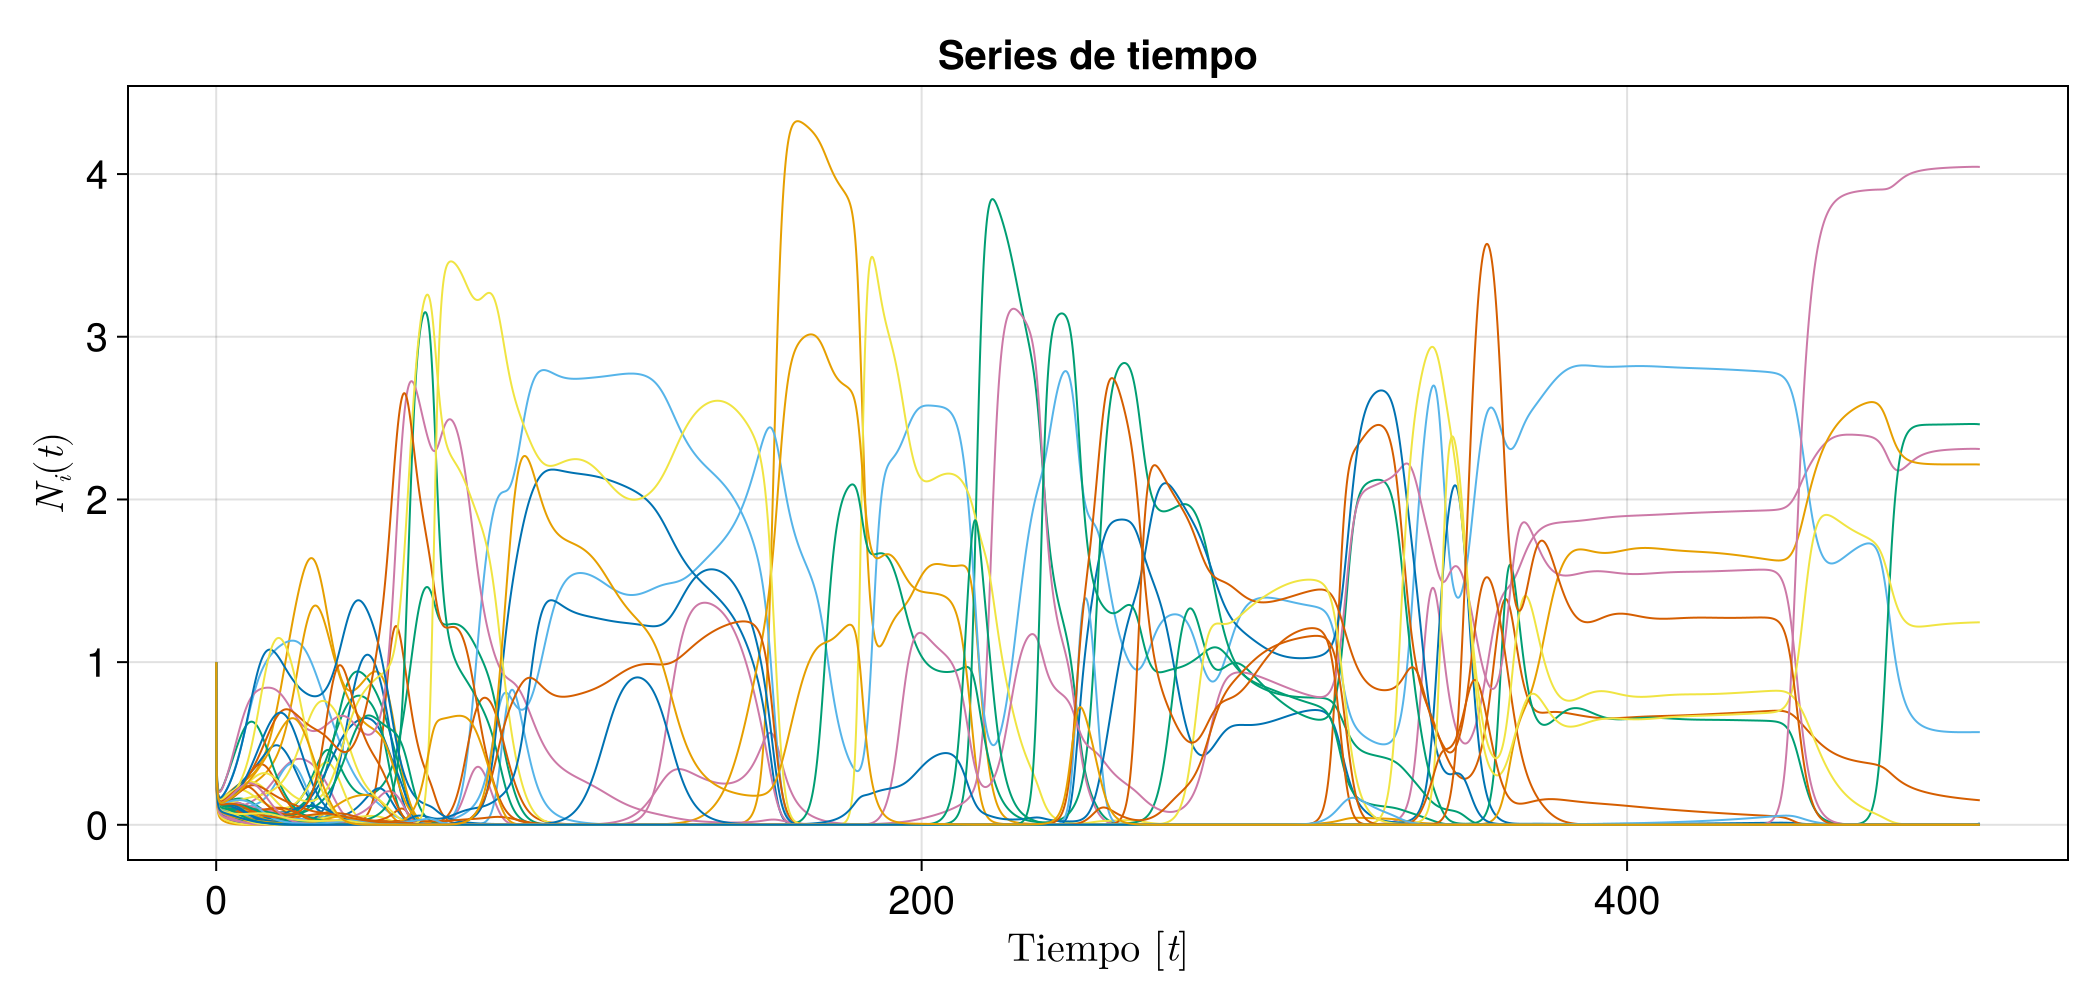
\includegraphics[scale=0.23]{../Imagenes/Seriesdetiempopositiva}
	\caption{Series de tiempo para el sistema de competencia de especies. Se emplea una matriz de incidencias de $100\times 100$ cuyas entradas son de una distribución uniforme en el intervalo [0,1]. En este caso particular no se considera a $\sigma$, solamente el tamaño de la red con $p=1.0$, es decir que es una red con el número máximo de enlaces posibles. En este caso la dinámica no sobrepasa la capacidad de carga puesto que las 100 especies se encuentran compitiendo y obedecen fielmente al comportamiento logístico.}
	\label{fig:Seriesdetiempopostiva}
\end{figure}

Una de las características que se encontró en esta clase de sistema en particular es que el tiempo en que tarda en estabilizarse es considerablemente mayor que en los sistemas donde consideraremos todas las interacciones antes mencionadas. Las poblaciones al estar confinadas por la capacidad de carga, tienen más oportunidad de interactuar entre sí pero esto genera que las constantes fluctuaciones prolonguen el tiempo de estabilización.
Por el contrario, el sistema generalizado sí excede la capacidad de carga lo que se traduce en una disminución de la cantidad de fluctuaciones que hace que el sistema pueda llegar al atractor en un tiempo mucho menor. Otro aspecto que se encontró en la red de competencias es que cuando es más conectada, tarda más tiempo en estabilizarse. Si generáramos una red de competencias con pocas conexiones ($p\leq 0.5$), el número de especies que compiten es considerablemente menor lo que produce que existan menor cantidad de fluctuaciones y a su vez las dinámicas de las poblaciones sean menos caóticas lo que hace que se pueda llegar a la estabilidad en un tiempo menor.\\
\\
En el Ejemplo \ref{eg:2x2CoopyDemás} del capítulo anterior, se observaba como las interacciones de cooperación $(--)$ en la matriz de incidencias $\Lambda$ genera la aparición de un atractor para ambas especies que se posiciona por arriba de la capacidad de carga (Figura (\ref{fig:CooperacionEspecies})). En el caso extendido a $N\gg 1$ especies ocurrirá lo mismo, solo que ahora tendremos un atractor $N$-dimensional. En este caso pueden haber especies que sobrepasen por mucho o poco la capacidad de carga, pero también cabe la posibilidad de que algunas no logren sobrepasarla y otras que lleguen a extinguirse. A continuación se muestran dos ejemplos diferentes
\begin{figure}[h!]
	\centering
	\includegraphics[scale=0.23]{../Imagenes/Series de Tiempo LK100}
	\caption{(\textbf{A}) Series de tiempo para el sistema de especies en competencia asociada a una matriz de incidencias de $100\times100$, con $\sigma=0.2$ y $p=0.35$. (\textbf{B}) Series de tiempo para el sistema de especies en competencia asociada a una matriz de incidencias de $100\times 100$ nodos con $\sigma=0.2$ y $p=0.5$}
	\label{fig:SeriesdeTiempoLK100}
\end{figure}

La diferencia evidente entre estas gráficas se da gracias a la matriz de incidencias, las interacciones que intervienen vienen de una fuerza de interacción promedio de $\sigma=0.2$ con diferentes probabilidades de conectividad, para $p=0.35$ y para $p=0.5$. El segundo caso corresponde con una red más conectada que el primero y eso se traduce al mismo tiempo en mayor oportunidad para crecer puesto que el crecimiento en este caso ronda hasta los 400 mientras que el otro escenario no pasa de 100. Esto podría interpretarse de la siguiente manera: entre más especies existan y cooperen entre sí, mayores serán sus crecimientos. Como se puede observar, el tiempo en que llegaron a estabilizarse fue menor a $t=50$, considerablemente menor a diferencia del caso de la Figura (\ref{fig:Seriesdetiempopostiva}). 

Sin embargo, el crecimiento no solamente depende de la cantidad de interacciones que existan (enlaces de la red), sino también de la fuerza de interacción promedio, entre mayor sea también se verá que la capacidad de crecimiento es proporcional a ello. Cuando se genera la matriz de incidencias en función de la matriz aleatoria (simétrica o no) y la matriz con entradas de una FDP normal centrada en $\mu=0$ se asume que existirán 50\% de valores positivos y 50\% de valores negativos distribuidos aleatoriamente en las 5 diferentes interacciones posibles\footnote{Si la matriz es puramente aleatoria son 5 posibles interacciones, sino entonces son 3.}. La presencia del comensalismo $(-0)$, depredación $(+-)$ o $(-+)$ y cooperación $(--)$ provoca numerosas especies logren superar la capacidad de carga del sistema para establecerse en el atractor $N$-dimensional, pero no hay que perder de vista que un ``exceso'' de estas interacciones genera inestabilidad y la posibilidad de que algunas de las especies divergan a infinito.
\\
\\
Los resultados de la Figura (\ref{fig:SeriesdeTiempoLK100}) en un principio se generaron a partir del tanteo y tomando como referencia la relación (\ref{eqn:parametroMay}), cabe preguntarse ¿cual debería se la cualidad de $\sigma$ y $p$ para que los sistemas de $N=100$ puedan hallar la estabilidad? La pregunta va encaminada a tratar de motivar la cualidad del parámetro crítico que relaciona $N$, $\sigma$ y $p$. Pero para llegar a ese punto primero se debe de conocer a la matriz de interacciones $\mathcal{I}$ resultante de realizar la integración del sistema y validar si lo que se nos muestra en estas gráficas de verdad es estabilidad (recordar la proposición \ref{prp:Atractores} acerca de la parte real de los eigenvalores de la matriz de interacciones).

\section{Matriz de interacciones}

En el capítulo anterior se definió el Jacobiano del sistema generalizado para poder determinar la matriz de interacciones, pero aún con ello no se ha presentado una forma de acceder a los puntos de equilibrio del sistema necesarios para dicho Jacobiano; debido a la naturaleza del sistema (considerando $N=100$), deben ser al menos 100 de ellos con diversas estabilidades. Calcularlos de manera analítica puede llegar a ser una tarea desafiante y poco redituable, pues de todos los puntos de equilibrio que puedan existir solo nos interesa el que es estable, y la mayoría de ellos podrían ser silla. La solución de ello por fortuna lo hallamos en el resultado de la integración numérica, como se puede ver en la Figura (\ref{fig:SeriesdeTiempoLK100}), al final de cada serie de tiempo se observa que las poblaciones llegan a estabilizarse. El último valor de cada población corresponde con una entrada del vector correspondiente al atractor que se encuentra contenido en el hiperespacio fase del sistema.\\
\\
Esto favorece a la construcción de los algoritmos que generan la matriz Jacobiana. Fácilmente se pueden programar las entradas de la matriz Jacobiana con base en la Definición \ref{def:MatrizInteracciones} y con ayuda de este vector correspondiente al atractor, se evalúa y finalmente se genera la matriz de interacciones $\mathcal{I}$ que tanto buscamos. Para tener certeza de la matriz de interacciones generada es importante validar que el sistema se estabiliza en un tiempo menor o igual (de preferencia menor) al tiempo final de la integración (en nuestro caso general para $t=50$). Se puede validar visualmente con las series de tiempo; una segunda validación sobre $\mathcal{I}$ es revisar que todos los elementos de su diagonal sean menores que cero, invocando así a la Proposición (\ref{prop:DiagonalI}. Se ha observado que cuando se ingresa un vector no correspondiente al punto de equilibrio estable, la diagonal de $\mathcal{I}$ contiene elementos positivos invalidando la proposición mencionada\footnote{Una hipótesis implícita de la Proposición \ref{prop:DiagonalI} es que para generar a $\mathcal{I}$ es necesario aplicar el Jacobiano de la Definición \ref{def:MatrizInteracciones} y evaluarlo en el atractor.}.
\\
\\
De esta forma podemos conocer las matrices de interacción de sistemas de competencia como los de la Figura \ref{fig:Seriesdetiempopostiva} y los sistemas generalizados de la Figura \ref{fig:SeriesdeTiempoLK100}. En este \href{https://github.com/rogve98/Tesis/tree/master/Notebooks/Datos/Ejemplo%20Jacobianos}{enlace}\footnote{Consultar: \url{https://github.com/rogve98/Tesis/tree/master/Notebooks/Datos/Ejemplo\%20Jacobianos}} el lector puede entrar a revisar por su cuenta el resultado de 4 matrices de interacción de sistemas que resultaron estables para los parámetros $N=100$, $\sigma=0.2$ y probabilidades $\{0.3,0.4,0.5,0.6\}$. Revisemos si en efecto estos ejemplos cumplen con la Poposición \ref{prop:DiagonalI}
\begin{tcolorbox}[colback=green!10!white, colframe=black, title=Entrada]
	\begin{minted}{julia}
using CSV, DataFrames
jacobianos = []
for i in 0.3:0.1:0.6
    ruta = "Datos/Ejemplo Jacobianos/Jacobiano100_p$i.s0.2.csv"
    df = CSV.read(ruta,DataFrame,header=false)
    push!(jacobianos,df)
end
jacobianos
	\end{minted}
\end{tcolorbox}

\begin{tcolorbox}[colback=red!10!white, colframe=black, title=Salida]
4-element Vector{Any}:\\
100×100 DataFrame
\end{tcolorbox}

Validando las diagonales de cada uno de las matrices de interacción consideradas se tiene

\begin{tcolorbox}[colback=green!10!white, colframe=black, title=Entrada]
	\begin{minted}{julia}
using LinearAlgebra
print(all(x -> x<0,diag(Matrix(jacobianos[1]))),", ")
print(all(x -> x<0,diag(Matrix(jacobianos[2]))),", ")
print(all(x -> x<0,diag(Matrix(jacobianos[3]))),", ")
print(all(x -> x<0,diag(Matrix(jacobianos[4]))))
	\end{minted}
\end{tcolorbox}

\begin{tcolorbox}[colback=red!10!white, colframe=black, title=Salida]
true, true, true, true
\end{tcolorbox}

El aspecto más importante de todas las matrices de interacción resultantes es que la diagonal no es homogénea como sí lo es en las matrices de May. Ocupando nuestro arreglo de Jacobianos veamos como son las disribuciones de los eigenvalores mediante la graficación de un histograma
\begin{figure}[h!]
	\centering
	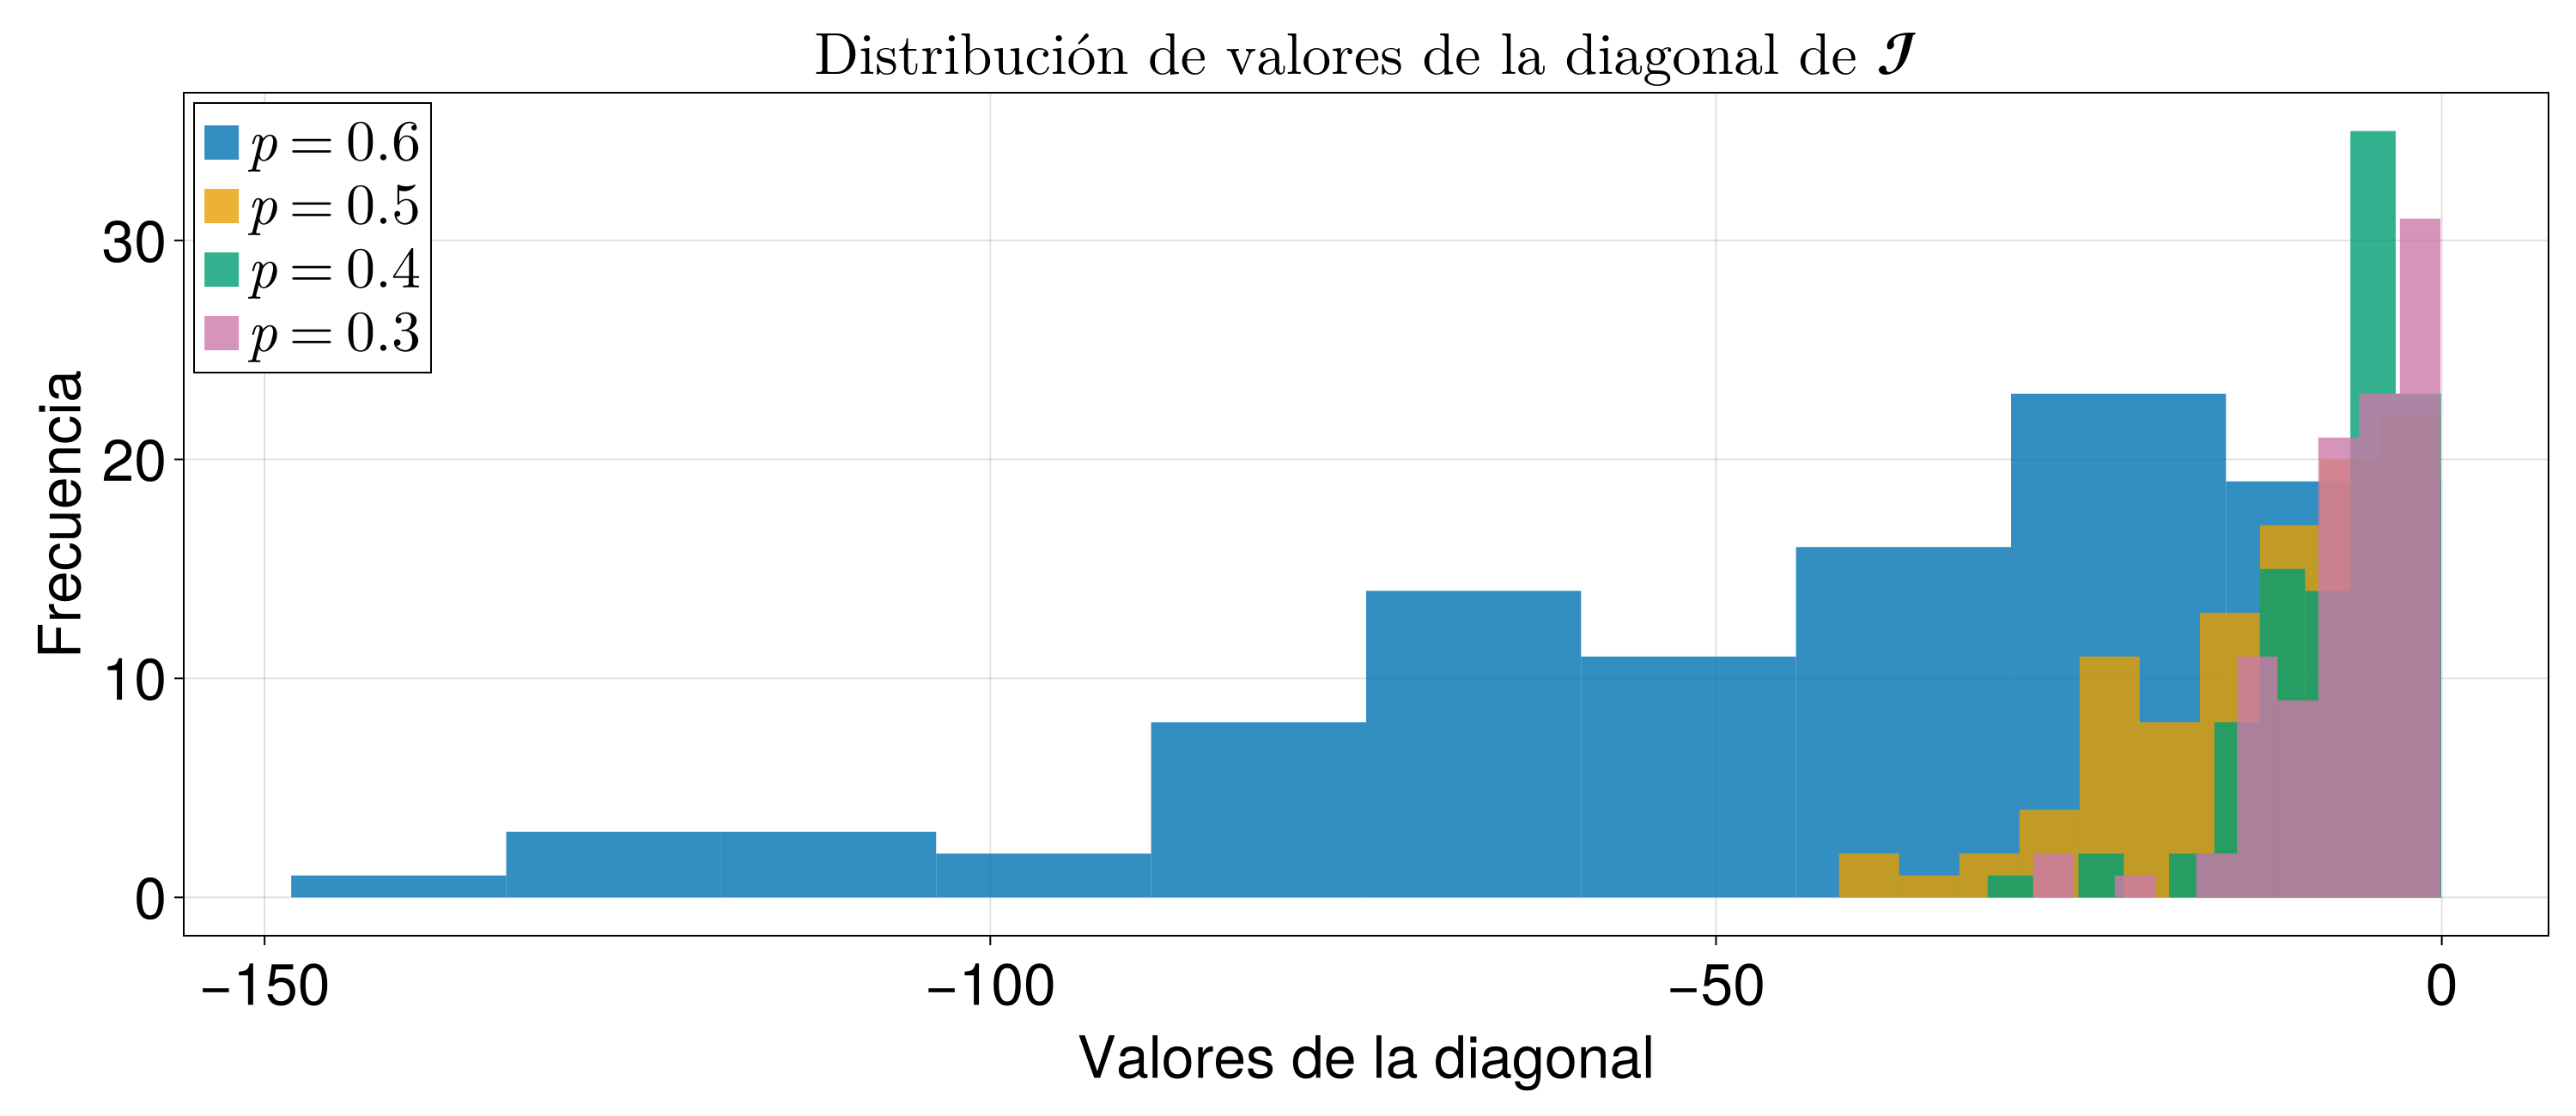
\includegraphics[scale=0.16]{../Imagenes/DistDiagonal}
	\caption{Distribución de la diagonal en matrices de interacción $\mathcal{I}$ del sistema generalizado para $N=100$, $\sigma=0.2$ y $p\in\{0.3,0.4,0.5,0.6\}$.}
	\label{fig:DistDiagonal}
\end{figure}

No solo no es homogénea sino que cuanto la probabilidad es mayor, la distribución es más dispersa hacia los valores negativos tal y como ocurre en el caso de $p=0.6$ en contraste con $p=0.3$. Este comportamiento es natural considerando el proceso de modelación e integración del sistema generalizado; suponer la diagonal homogénea es establecer un sistema demasiado ideal y por tanto difícilmente aproximable a la realidad. Esta propuesta pretende acercarse hacia la dinámica que presentan sistemas semejantes a la realidad, sin embargo aún sigue siendo muy teórico. 
\\
\\
En el capítulo pasado se vio que la importancia de la diagonal radica en la forma de la distribución de los eigenvalores del sistema en el plano complejo, englobado bajo la Ley Circular. En las matrices de May, la diagonal representaba el centro y radio del círculo que encerraba esta distribución de eigenvalores; a partir de esta distribución se puede visualizar de otra forma si el sistema es estable o no, viendo el signo de la parte real de los mismos. En nuestro caso, al no tener un radio/centro definido ¿qué podemos esperar de la distribución de eigenvalores de $\mathcal{I}$?
\newpage

\section{Leyes Circulares}

Viendo que la distribución de la diagonal no es homogénea en los sistemas generalizados, se debe analizar como es la distribución de lo eigenvalores en el plano complejo y si podría seguir la Ley Circular que establece May. Para ello se comenzará por revisar la distribución de eigenvalores de las matrices de interacción $\mathcal{I}$ que se invocaron en la sección anterior
\begin{figure}[h!]
	\centering
	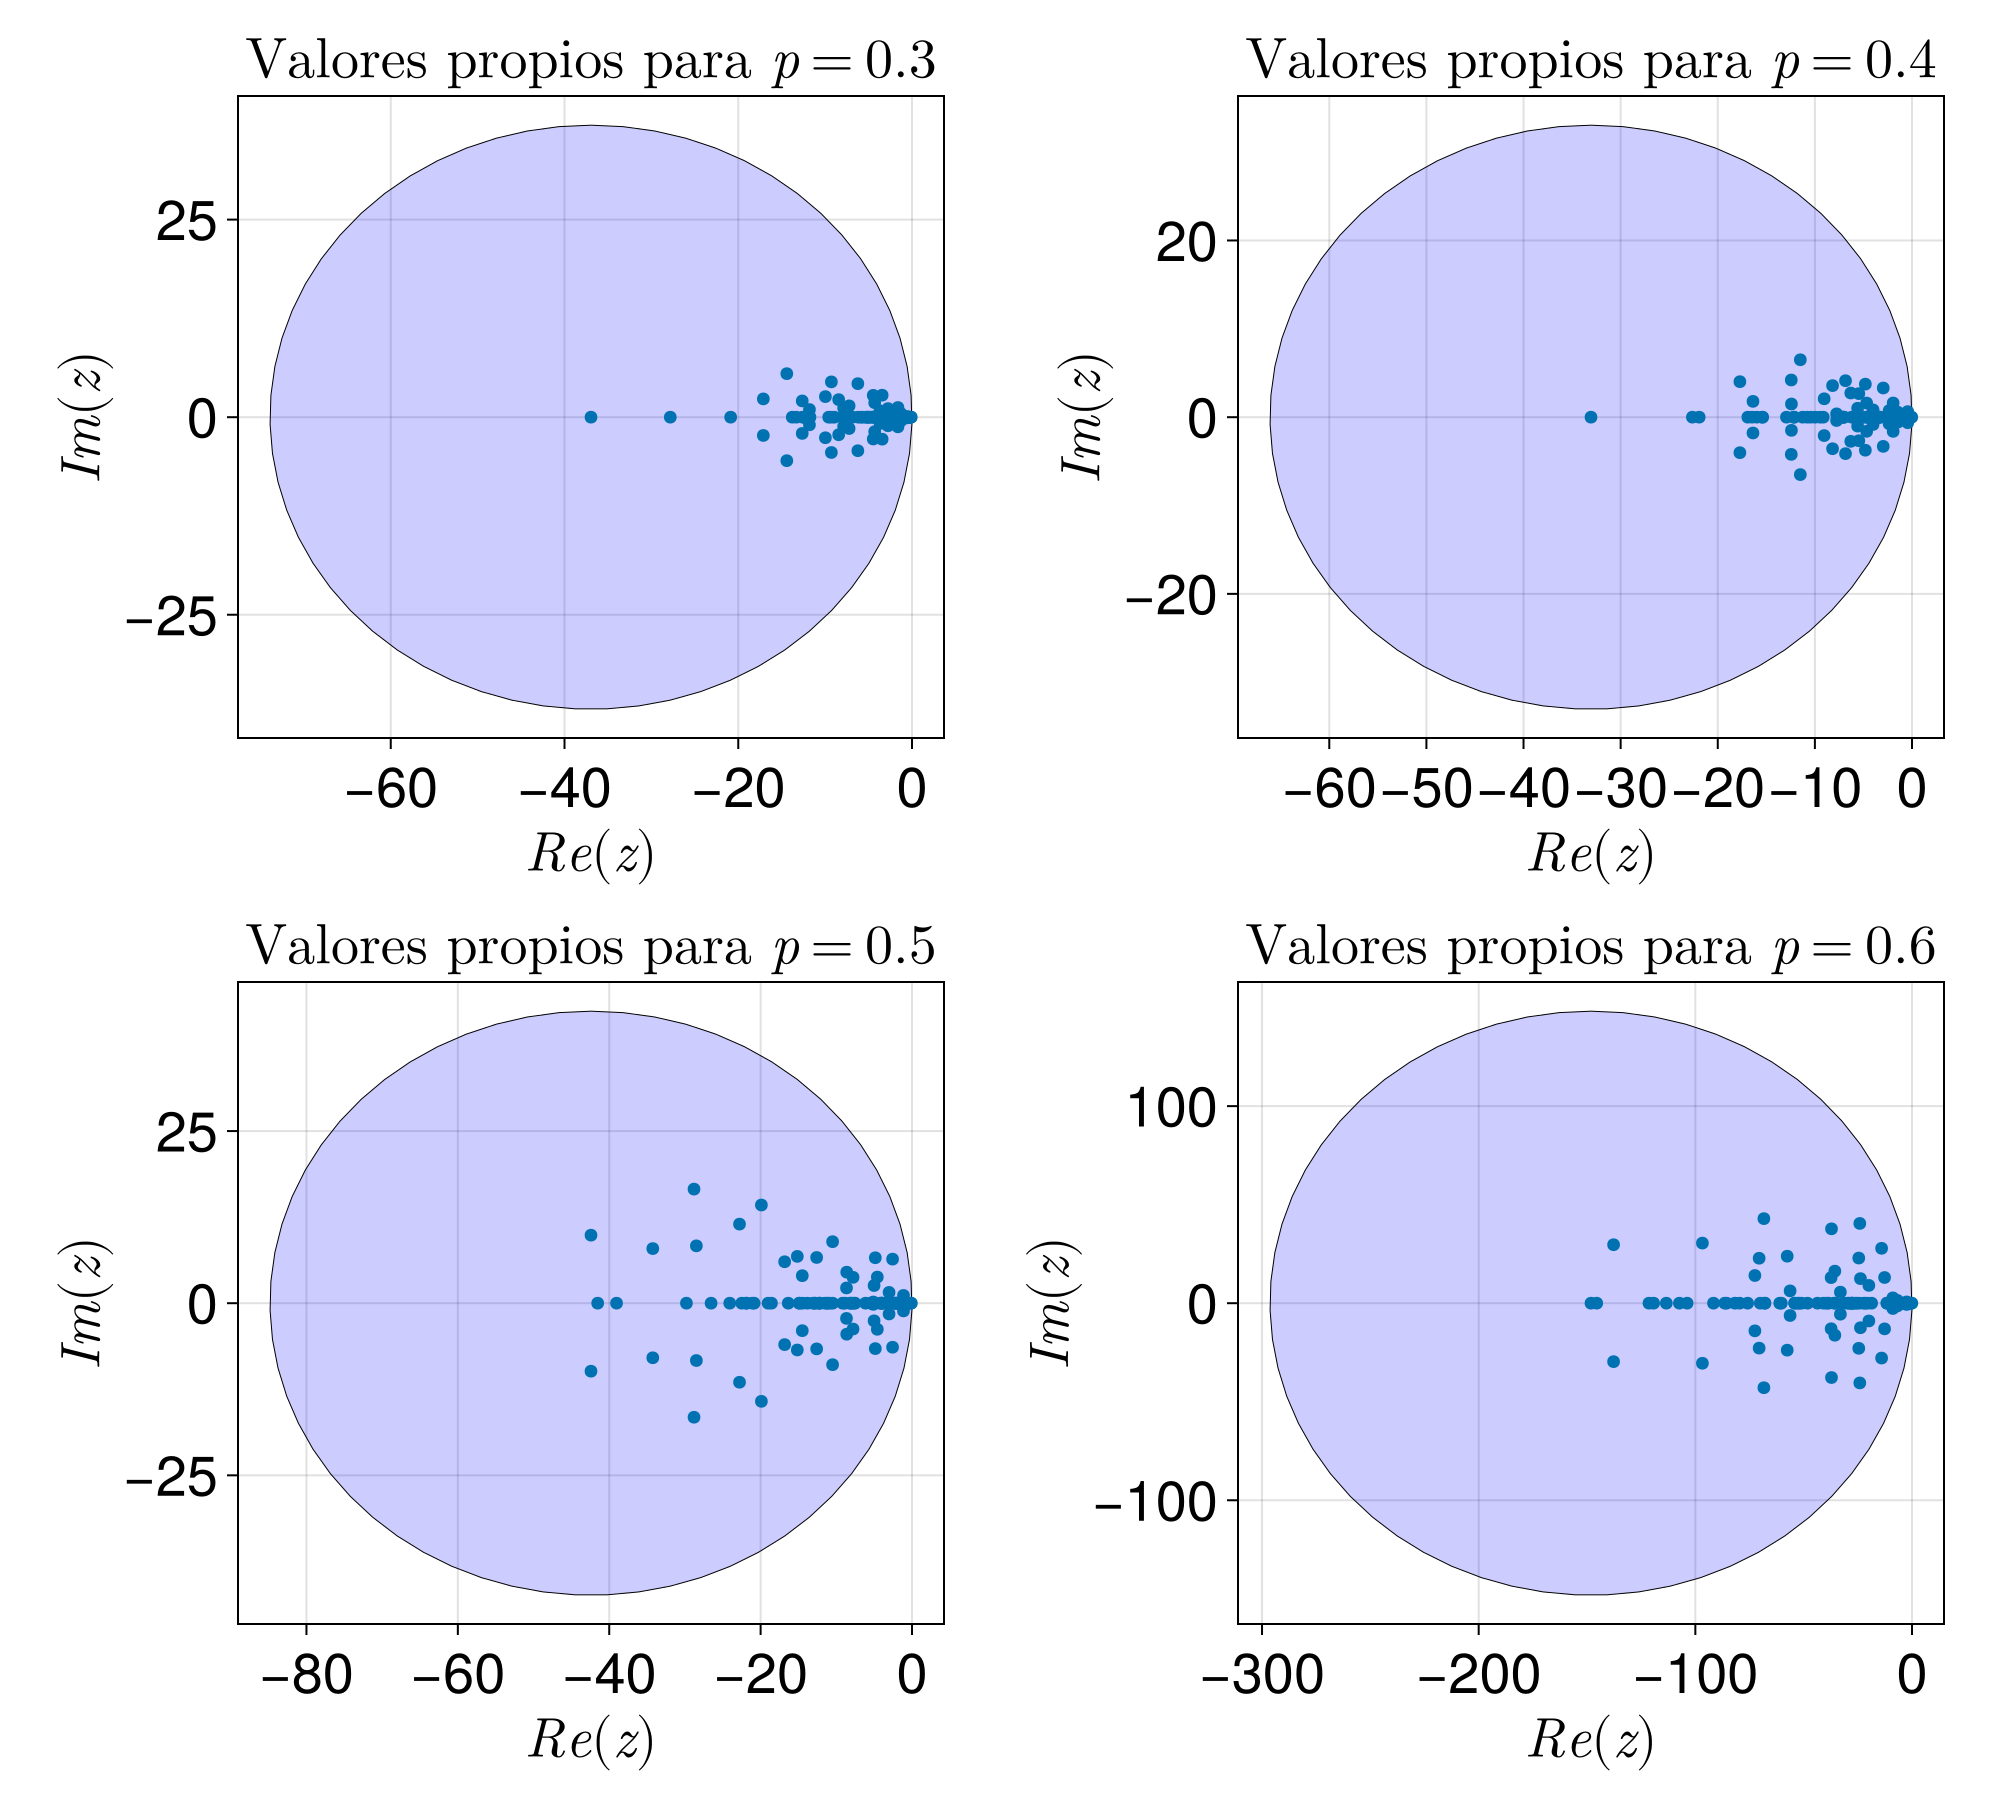
\includegraphics[scale=0.24]{../Imagenes/DistEigenvalores}
	\caption{Distribución de eigenvalores para el conjunto de jacobianos con los parámetros $N=100$, $\sigma=0.2$ y $p\in\{0.3,0.4,0.5,0.6\}$.}
	\label{fig:DistEigenvalores}
\end{figure}

Para comenzar, se ha propuesto el centro/radio como el eigenvalor con parte real mínima de cada distribución\footnote{En consecuencia se genera el Círculo con el radio más grande posible de cada sistema.}, y en primera instancia se puede observar que dicho círculo si encierra a toda la distribución de eigenvalores, además también se puede notar que en cada caso los eigenvalores cuentan con parte real negativa lo que sustenta que cada sistema sea estable. Sin embargo es notorio que la distribución no se ajusta al círculo resultante sino solamente a una parte del mismo. Otro aspecto que se puede apreciar de esta distribución es que cuanto mayor es la probabilidad de conexión entre nodos, la distribución se ensancha al igual que como ocurrió en la distribución de la diagonal Figura (\ref{fig:DistDiagonal}). \\
\\
El hecho de que la distribución de la diagonal no sea homogénea impacta directamente en la distribución de los eigenvalores, pero ¿qué pasa si en lugar de proponer una sola Ley Circular, se proponen $N$? Para ello se ocupará la distribución más ancha, con $p=0.6$ y se considerará cada valor de la diagonal de su matriz de interacciones $\mathcal{I}$ como centro y radio de una Ley Circular particular
\begin{figure}[h!]
	\centering
	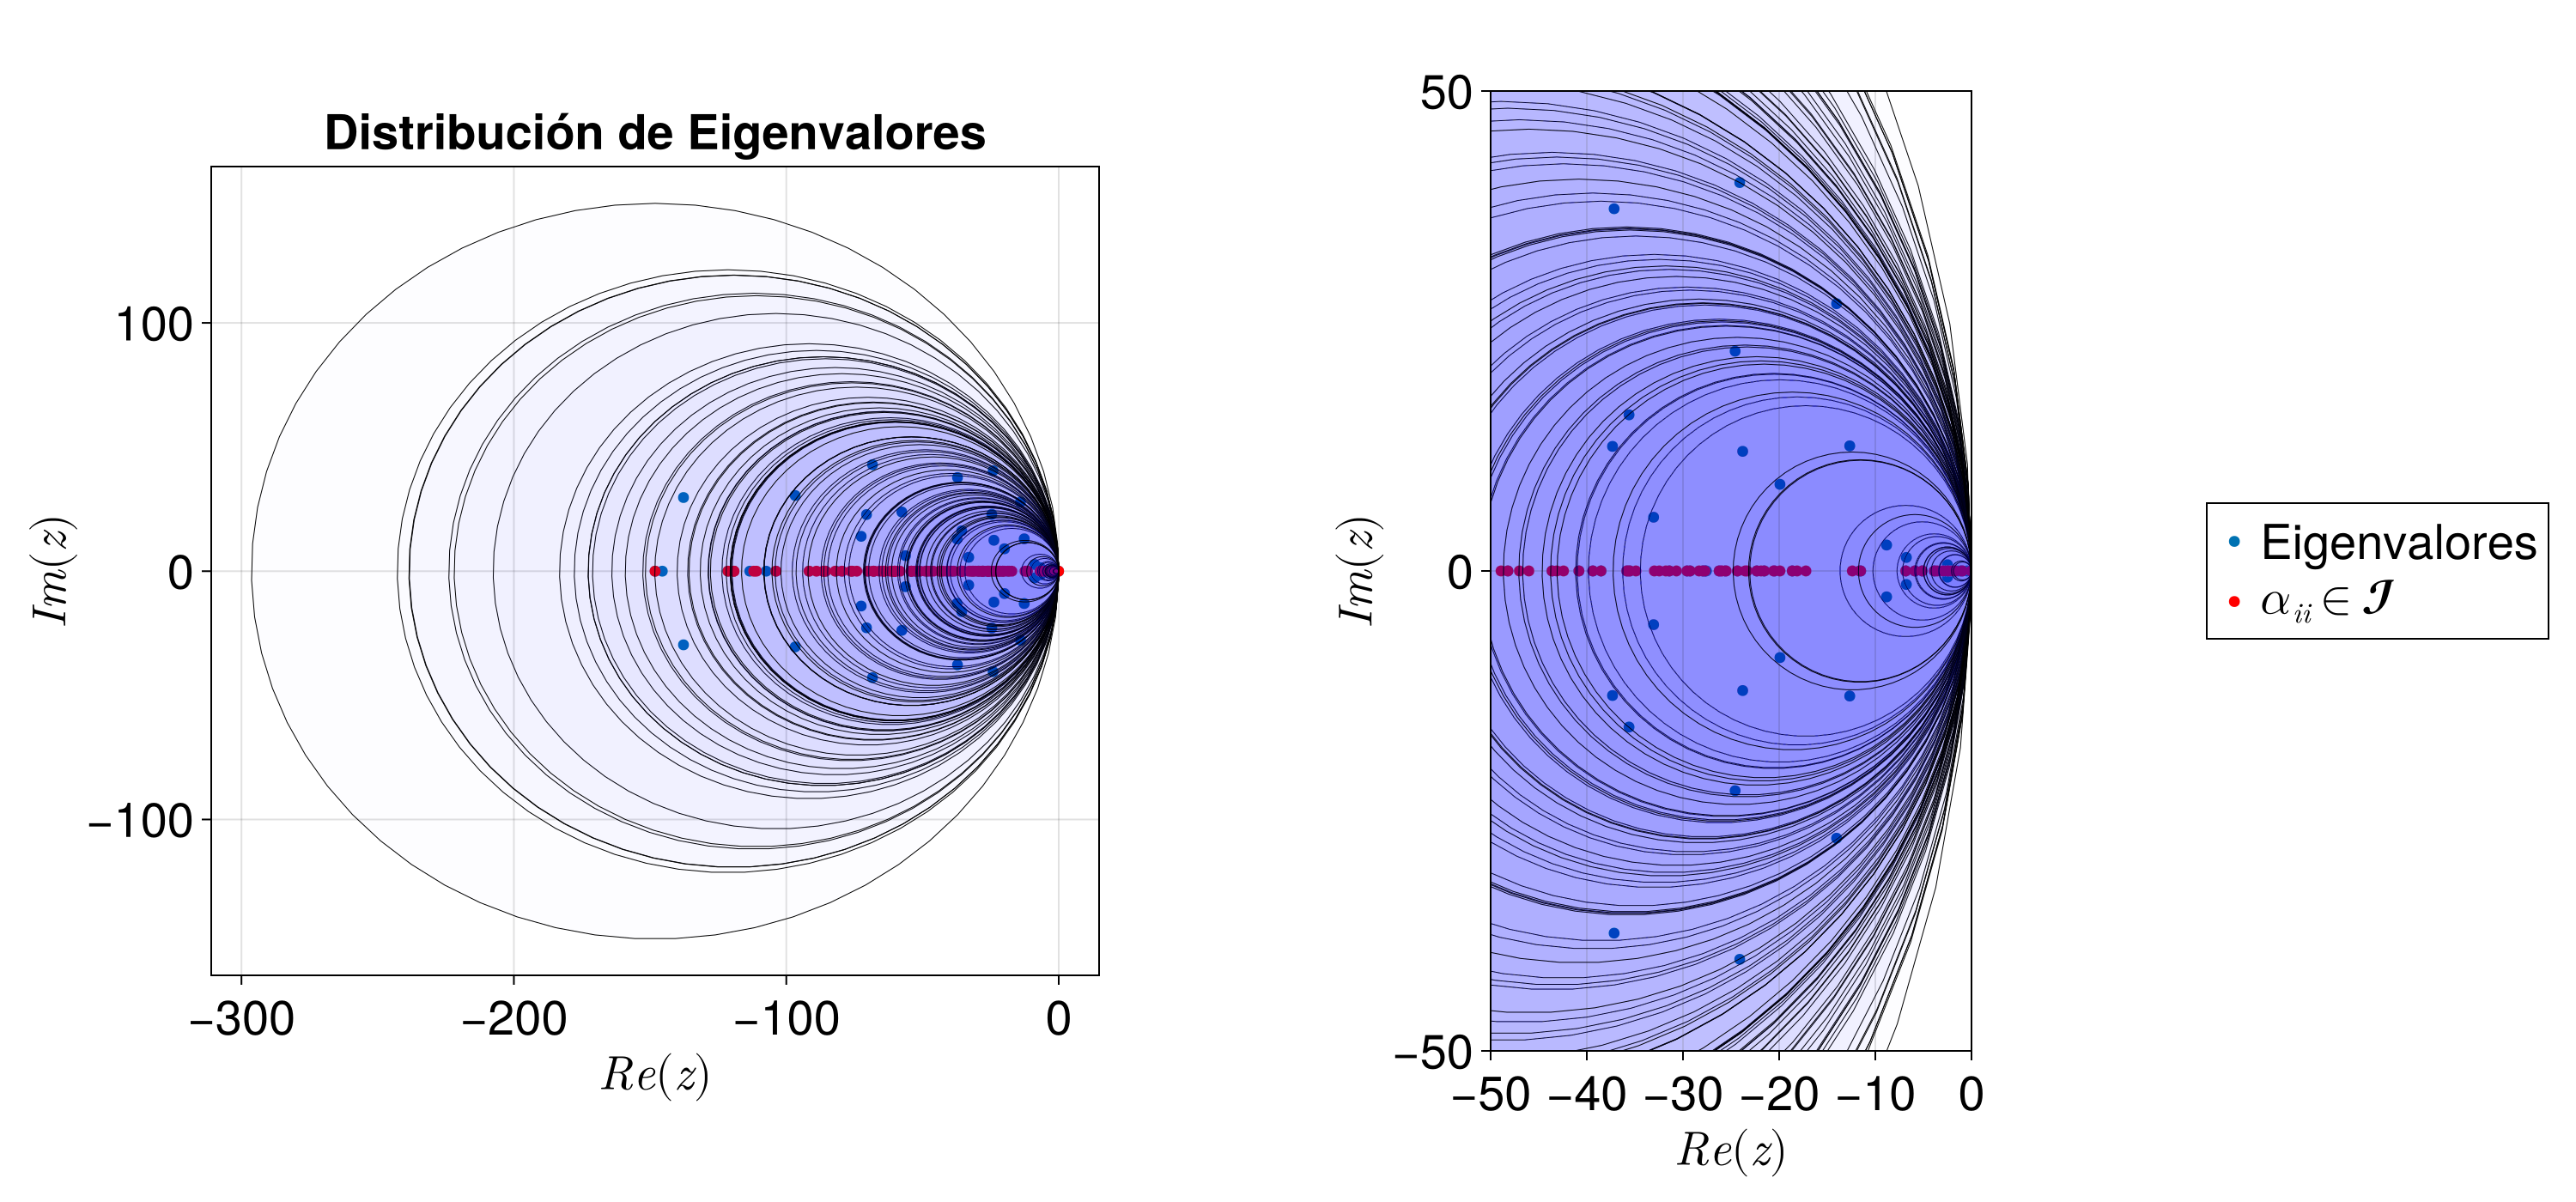
\includegraphics[scale=0.17]{../Imagenes/LeyesCirculares}
	\caption{Distribución de eigenvalores del sistema generalizado para $N=100$, $\sigma=0.2$ y $p=0.6$. Se consideran $N$ Leyes Circulares cuyo radio y centro es cada valor de la diagonal de la matriz de interacciones $\mathcal{I}$ asociada. }
	\label{fig:LeyesCirculares}
\end{figure}

Esta propuesta sugiere que cada valor de la diagonal funge como un centro y radio de una Ley 
\begin{wrapfigure}{l}{0.5 \textwidth} \vspace{-30pt} \begin{center}
	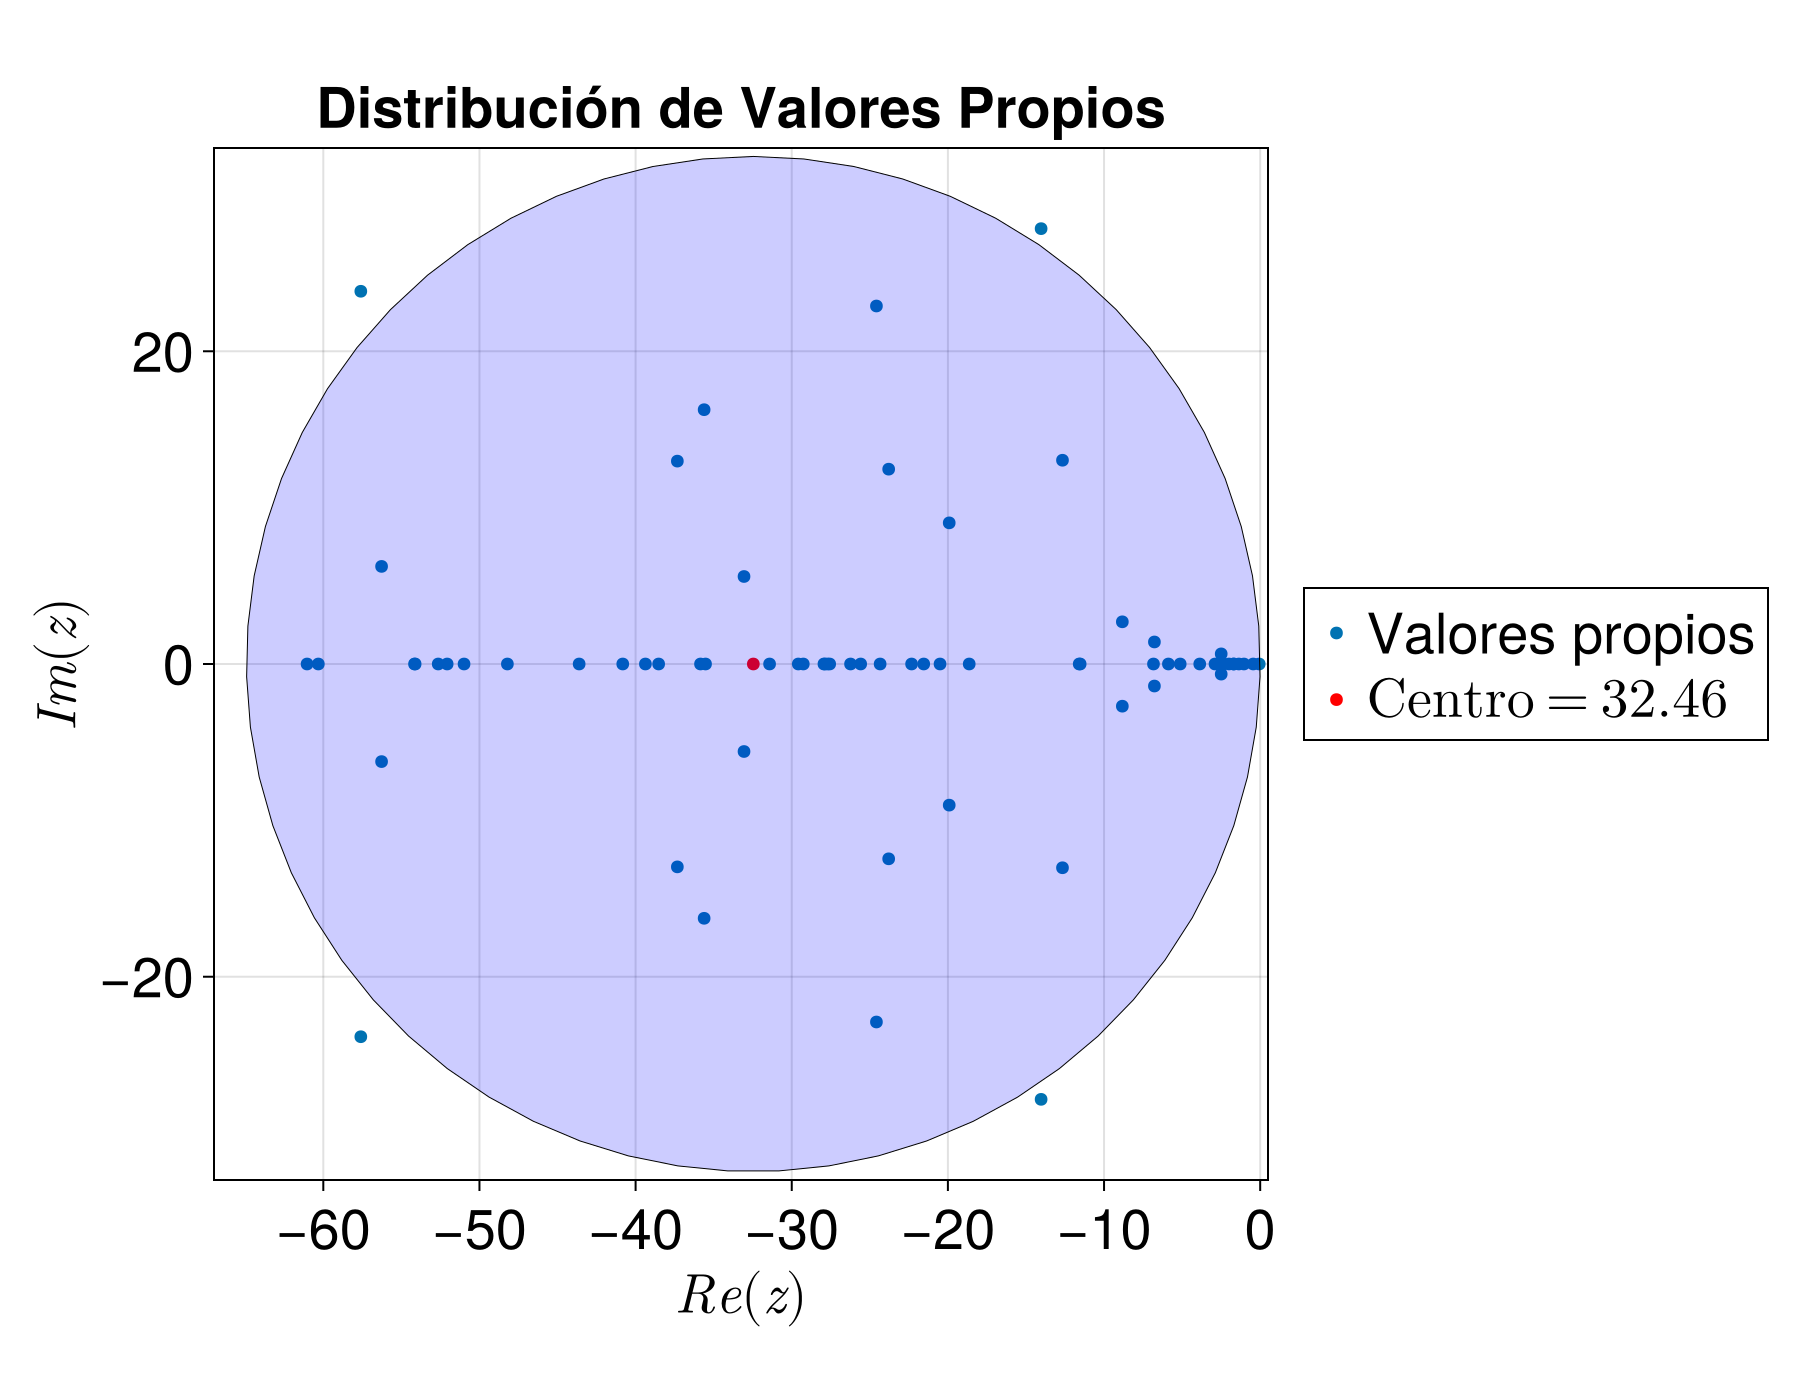
\includegraphics[scale=0.13]{../Imagenes/LeyCircularParticular}
	\end{center}
	\vspace{-20pt} 
	\caption{Caso particular de la Figura (\ref{fig:LeyesCirculares}) para el valor de la diagonal $\alpha_{ii}=32.46\in\mathcal{I}$.}
		\vspace{-10pt}
	\label{fig:LeyCircularParticular}
\end{wrapfigure}
Circular local que encierra cierta cantidad de eigenvalores mismos que se ajustan a dicho círculo particular. Hemos visto el mínimo valor de la distribución de la diagonal genera un Círculo que encierra a todos los eigenvalores pero no necesariamente la distribución se ajusta a este círculo más grande. En resumen, la propuesta que aquí se genera es que la distribución de eigenvalores de un sistema generalizado se ajusta a $N$ Leyes Circulares, mismas que se generan a partir de los valores de la diagonal de $\mathcal{I}$. De la Figura (\ref{fig:LeyesCirculares}) analicemos más de cerca un caso particular para el valor de la diagonal $\alpha_{ii}=32.46$ (Figura \ref{fig:LeyCircularParticular}), gran parte de los eigenvalores no tienen parte imaginaria sino solo la parte real negativa mientras que el resto se distribuye por el resto del círculo a excepción de algunos otros eigenvalores que pasan al siguiente nivel o siguiente círculo. Para poder confirmar o refutar esta propuesta, se necesitan de más eigenvalores dibujados en el plano complejo, ya que los eigenvalores de un solo sistema nos brinda información limitada.

\subsection{Análisis para $N=50$}

Como parte de la investigación, se tienen  a disposición un banco de \href{https://github.com/rogve98/Tesis/tree/master/Notebooks/Datos/Jacobianos}{Jacobianos} y otro de \href{https://github.com/rogve98/Tesis/tree/master/Notebooks/Datos/Diagonales}{Diagonales}\footnote{Para los Jacobianos acceder a: \url{https://github.com/rogve98/Tesis/tree/master/Notebooks/Datos/Jacobianos}. Para las Diagonales acceder a \url{https://github.com/rogve98/Tesis/tree/master/Notebooks/Datos/Diagonales}.} de Jacobianos en donde se concentran 78 archivos .csv en cada banco, y contienen cada uno la información de 100 simulaciones diferentes que resultaron ser estables. Debido al costo computacional, se tuvieron que generar para $N=50$ para los siguientes casos:
\begin{table}[h!]
	\centering
	 \begin{tabular}{|c|c|c|c|}
		\hline
		Valor promedio [$\sigma$] & Probabilidades [$p$] & Cantidad de archivos & Simulaciones realizadas \\ \hline
		$0.1-0.5$  & $0.1-1.0$  & 50 & 5000  \\ \hline
		0.6  & $0.1-0.9$  & 9 & 900 \\ \hline
		0.7  & $0.1-0.7$  & 7 & 700 \\ \hline
		0.8  & $0.1-0.5$  & 5 & 500 \\ \hline
		0.9  & $0.1-0.4$  & 4 & 400 \\ \hline
		1.0  & $0.1-0.3$  & 3 & 300 \\ \hline
		& \textbf{Total:} & 78& 7800\\ \hline
	\end{tabular}
	\caption{Cantidad de archivos generados para el banco de Diagonales y Jacobianos considerando $N=50$. A partir de $\sigma=0.6$ en adelante, los tiempos de compilación fueron muy prolongados por lo que no se obtuvieron los 10 archivos respectivos a diferencia de los valores promedio anteriores.}
	\label{tab:Simulaciones}
\end{table} 

La razón de explorar sistemas estables para valores de $\sigma$ y $p$ cercanos a 1.0 era para ver que tan probable era que fueran estables en estas condiciones, además de obtener un mínimo de información posible para fortalecer el análisis que se hará a continuación. Se busca realizar una caracterización de las distribuciones enfocándose principalmente en la relación que tiene la media con la desviación estándar de cada una de las 7800 distribuciones; sobre todo ver de que forma cambia en función de los parámetros $\sigma$ y $p$. Con base en los resultados encontrados, se explorará si también existe una relación entre la distribución de las diagonales con la distribución de la parte real de los eigenvalores asociados a los sistemas estables, de esta forma se podrá justificar parcialmente la propuesta de las \textit{Leyes Circulares}, que indica que cada valor de la diagonal puede fungir como centro y radio de una de $N$ leyes circulares que encierran localmente cierta cantidad de eigenvalores del sistema.

\subsubsection*{Diagonales}

Algo que se ha visualizado en un primer acercamiento (Figura (\ref{fig:DistDiagonal})) es que cuando es más grande la conectividad del sistema (parámetro $p$), la distribución de la diagonal es más amplia. Se confirmará esto con los datos disponibles y además se verá si ocurre algo similar para $\sigma$ en las mismas circunstancias. A continuación se revisará de forma cualitativa la forma de algunas distribuciones de diagonales asociadas a ciertas $p$ y $\sigma$ con $N=50$
\begin{figure}[h!]
	\centering
	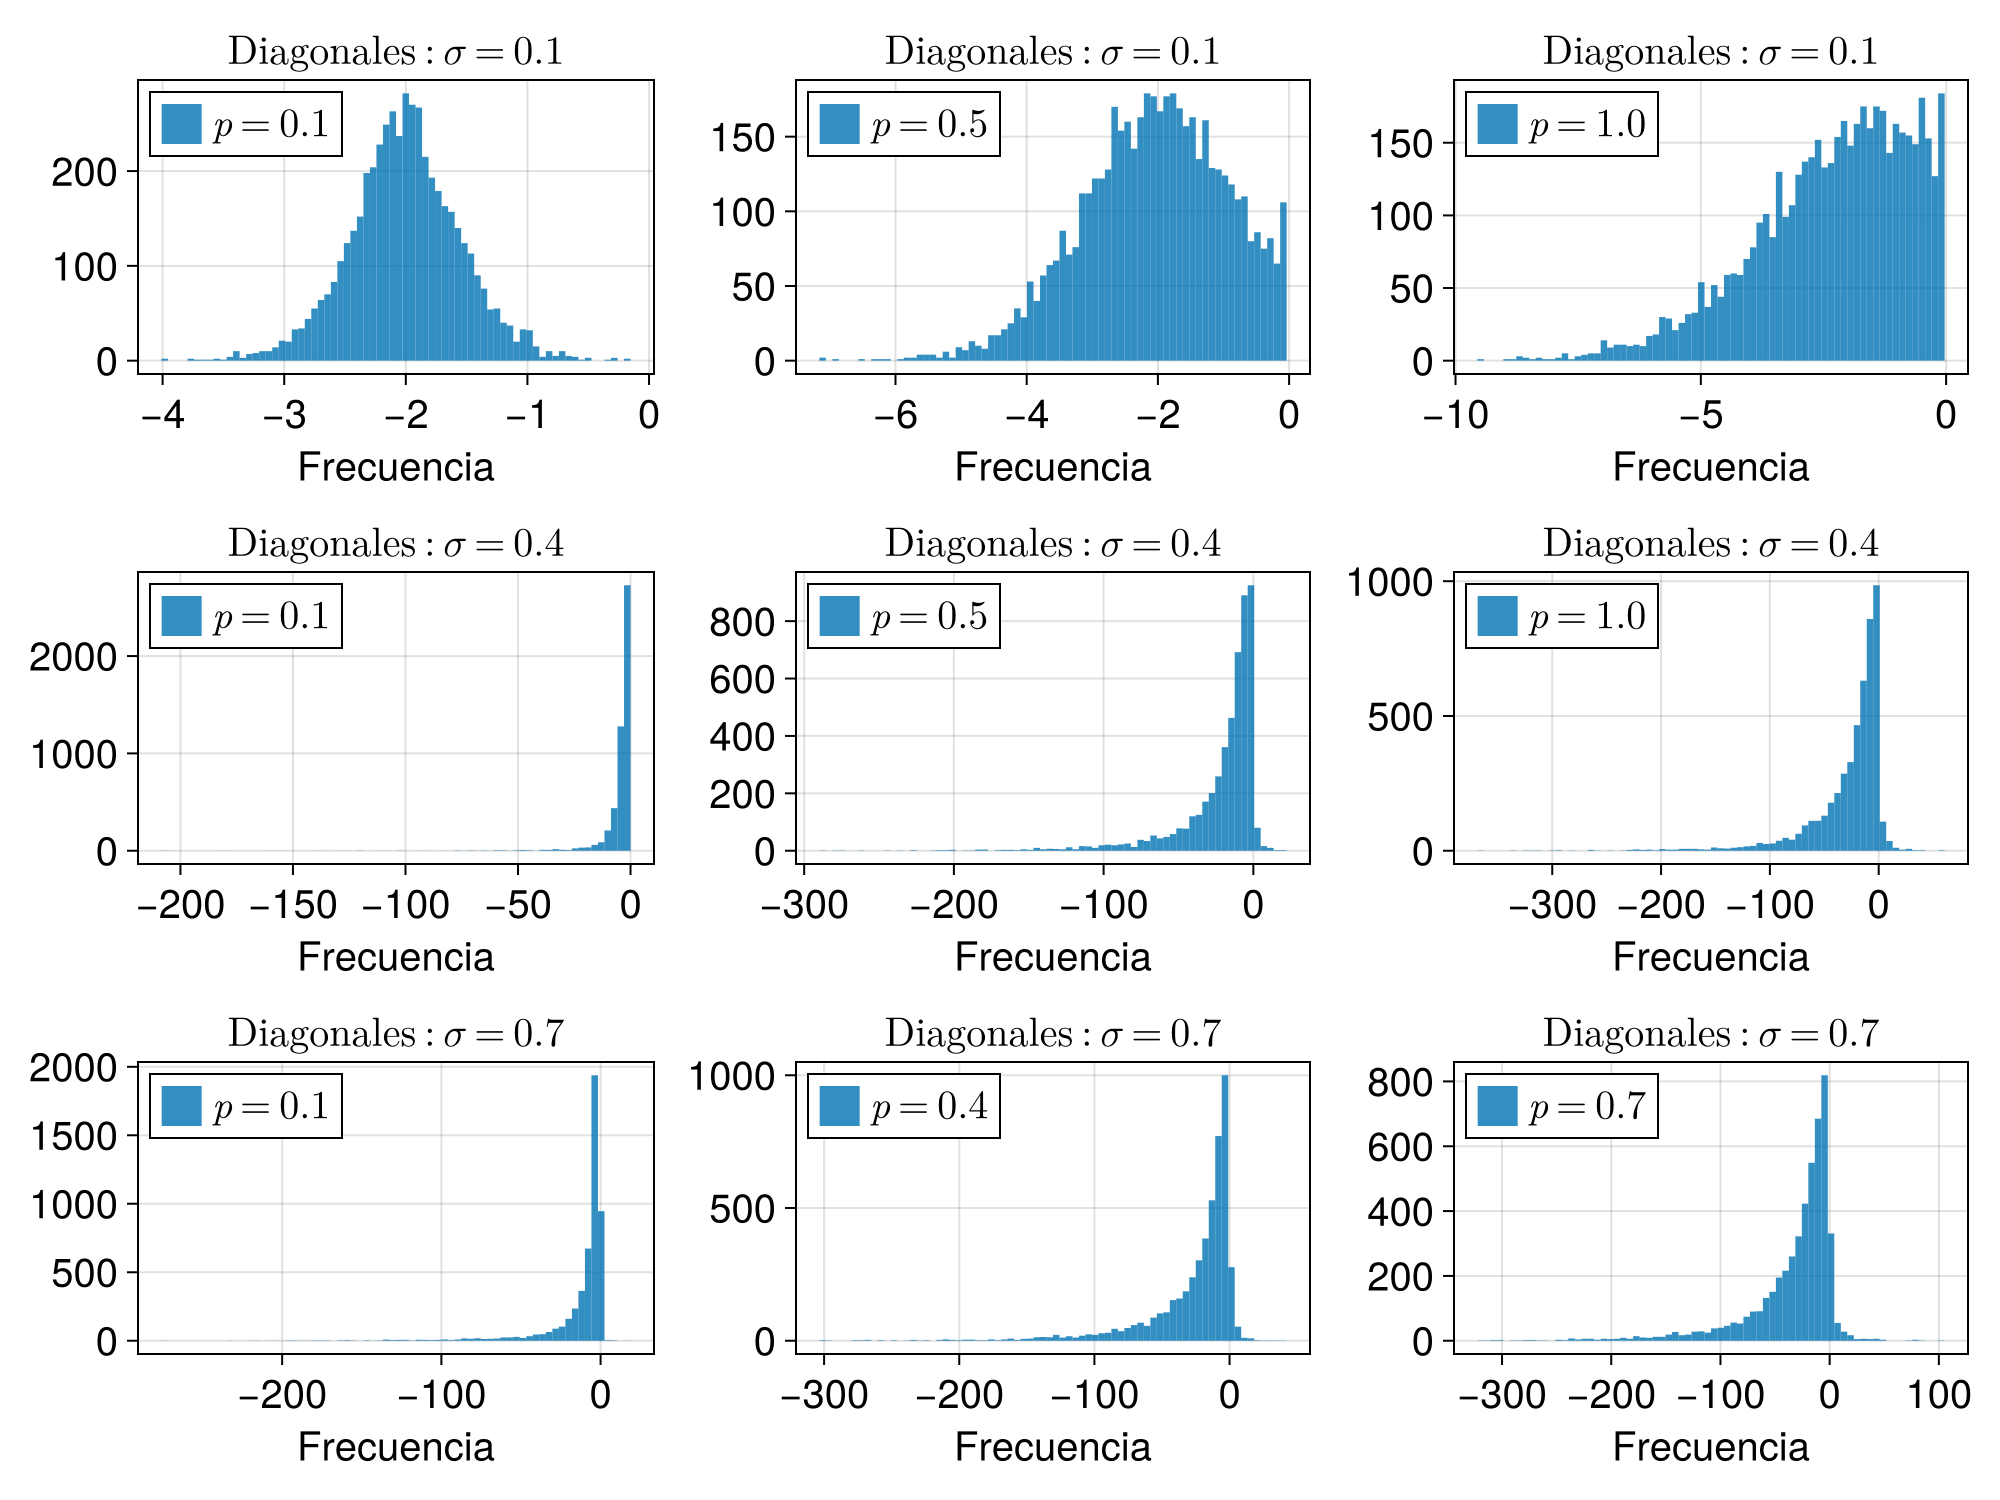
\includegraphics[scale=0.24]{../Imagenes/distDiagonales50}
	\caption{Distribución de 500 diagonales resultantes de 100 sistemas estables/cuasi-estables para $N=50$. Cuando $\sigma$ y $p$ tienden hacia 1, aumenta la tendencia hacia distribuciones de cola pesada.}
	\label{fig:distDiagonales50}
\end{figure}

Se puede observar que la distribución de las diagonales tiene una tendencia FDP normal para los casos con $\sigma=0.1$, sin embargo conforme las probabilidades aumentan, haciendo que los sistemas sean cada vez más conectados, la distribución se va ensanchando y sesgando hacia la izquierda. Para los casos $\sigma=0.2$ en adelante, se sigue una tendencia de distribución de cola pesada. Las distribuciones al no ser simétricas, indican que la media estadística $\langle d_{kk}(\sigma_i,p_j)\rangle$ se encuentra hacia la izquierda de la moda estadística. Para cada $\sigma$ se observa que a medida que $p$ aumenta, la distribución se ensancha siendo cada vez más dispersa; por lo tanto la media estadística se va desplazando hacia la parte negativa a medida que la desviación estándar $s(d_{kk}(\sigma_i,p_j))$ es más grande.
\\
\\
Cuando se observa que las distribuciones son más compactas, entonces la media puede encontrarse en un valor más cercano al cero. Esto puede indicar que existe una correlación entre ambas medidas estadísticas por lo que se tendría que comprobar este hecho. La forma de la distribución de las diagonales puede asemejarse a la distribución Log-Normal que es bien conocido que tiene una relación no trivial entre su media y desviación estándar [cita\footnote{Cita}], sin embargo, al realizar los ajustes correspondientes, se encuentra que el $p$-valor es suficientemente cercano a cero como para descartar esta hipótesis. \\
\\
Debido a ello solamente se asumirá que es una distribución con sesgo negativo. Se ha determinado un ajuste lineal ``general'' para las 7800 simulaciones únicamente para notar si el comportamiento es 
\begin{wrapfigure}{r}{0.5 \textwidth} \vspace{-20pt} \begin{center}
		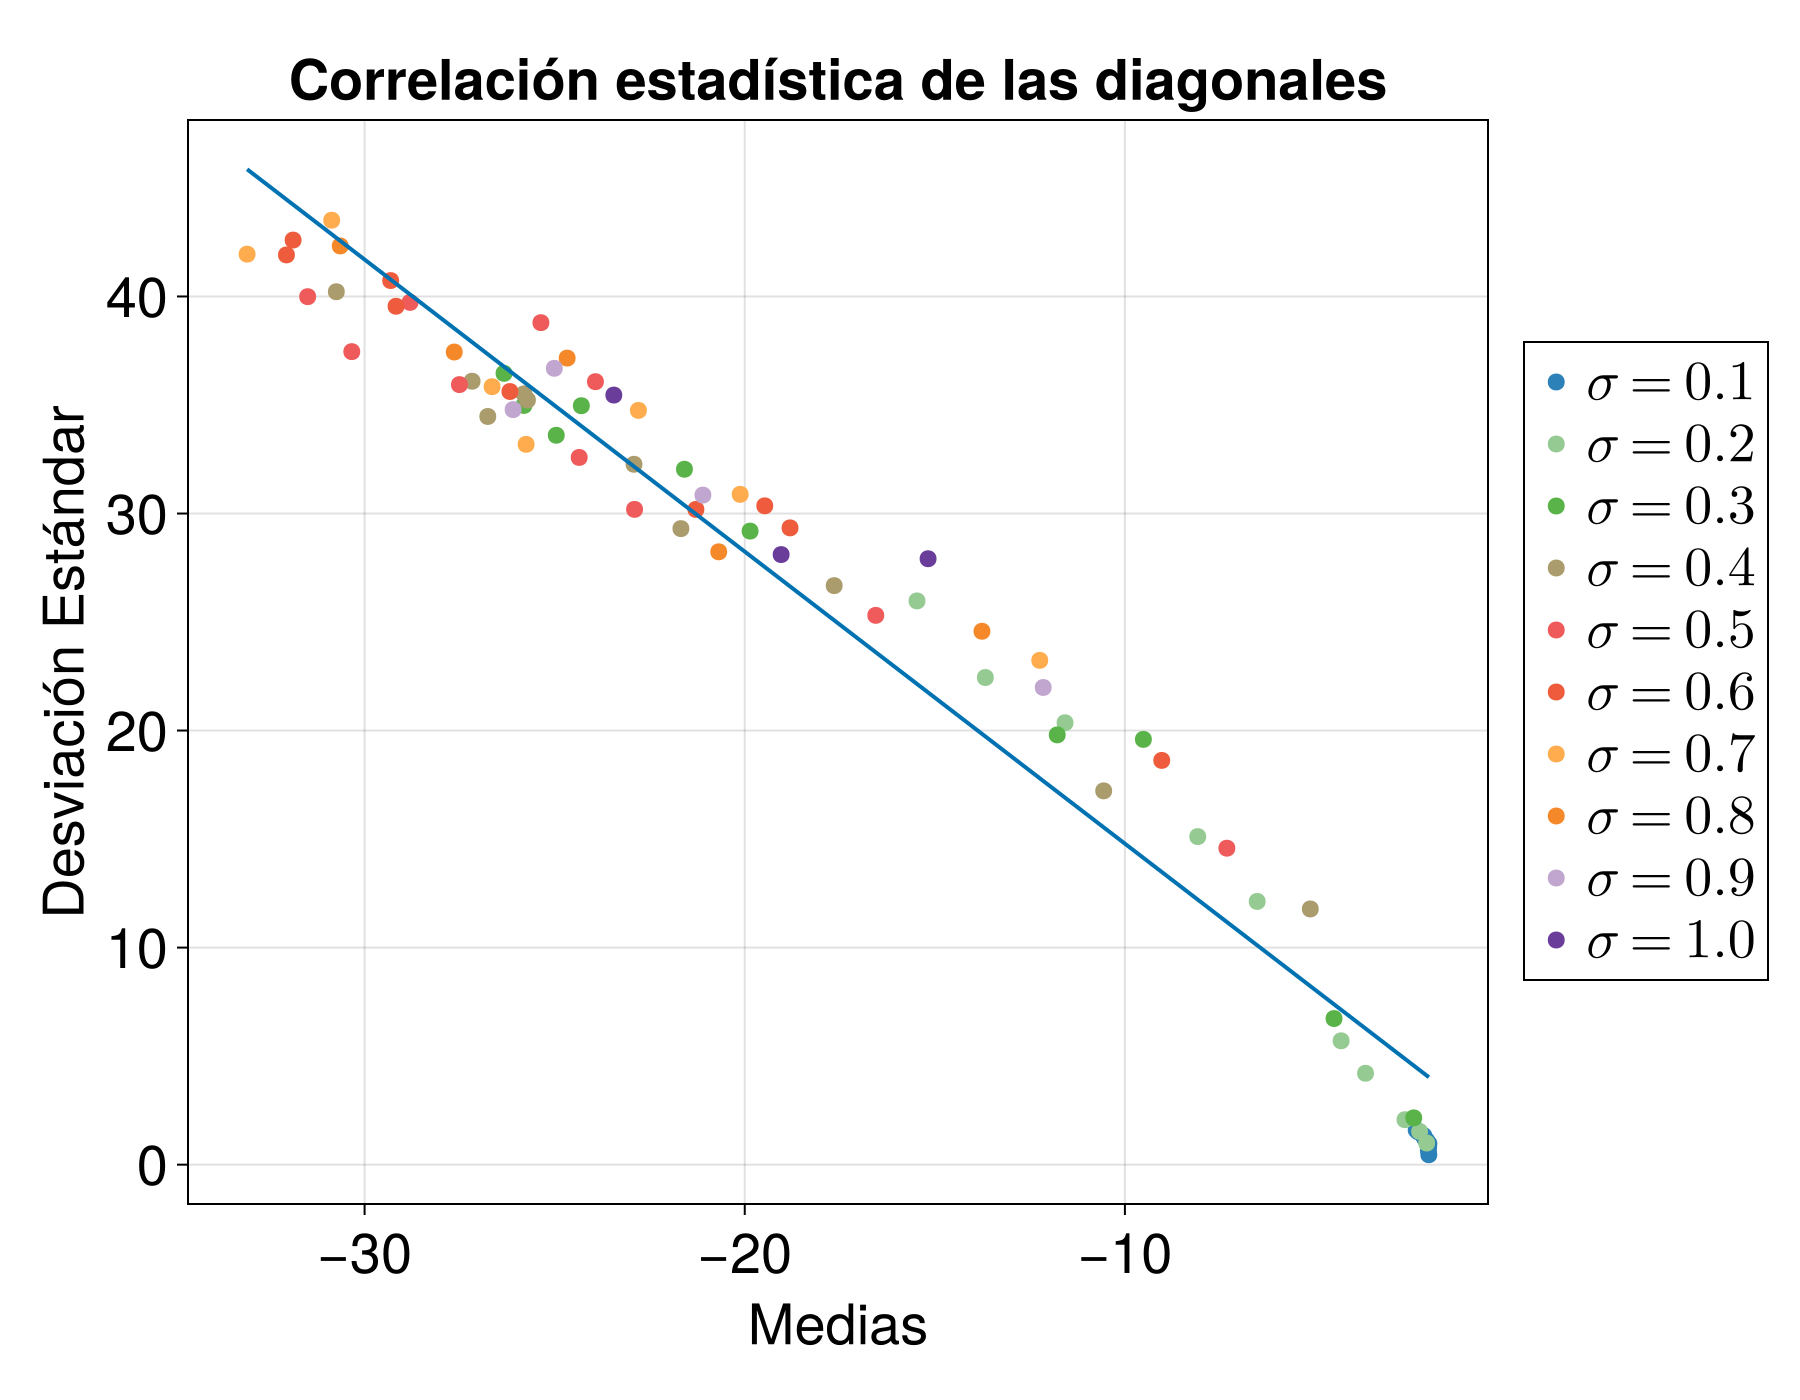
\includegraphics[scale=0.15]{../Imagenes/CorrelacionMvsStd}
	\end{center}
	\vspace{-20pt} 
	\caption{Ajuste lineal entre los promedios y las desviaciones estándar de cada una de las 7800 simulaciones realizadas bajo los parámetros que dicta la Tabla (\ref{tab:Simulaciones}).}
	\vspace{-10pt}
	\label{fig:CorrelacionMvsStd}
\end{wrapfigure}
compartido entre diferentes parámetros de $\sigma$ y $p$. Cada color corresponde con una $\sigma$ definida y las probabilidades se distinguen a partir de la media/desviación estándar, entre más grande sea el valor de $p$ también será más grande la magnitud de las anteriores. El comportamiento general es que existe una relación lineal entre la media y la desviación estándar. Cuanto más grandes son $\sigma$ y $p$, la media se desplaza hacia los valores negativos y las distribuciones son cada vez más dispersas.
Habría de ejecutarse un ajuste lineal para cada $\sigma$, sin embargo, con los datos disponibles se puede determinar los coeficientes de correlación para cada $\sigma$ y corroborar de manera indirecta lo que nos anuncia la gráfica (Tabla (\ref{tab:Correlaciones})). Lo que se puede observar es que se tiene una muy fuerte correlación entre ambas cantidades estadísticas, a excepción de los casos $\sigma=\{0.1,1.0\}$ en donde se tienen los coeficientes bajos. \\
\\
El primer caso es muy especial ya que las observaciones indican que las distribuciones de diagonales pasan de ser simétricas (normal) a ser una distribuciones con sesgo negativo a medida que $p$ vaya aumentando. Realizando un ajuste lineal al caso $\sigma=0.1$ se podrá ver que no es tan bueno como en el resto de los casos, muy posiblemente se deba a esta evolución hacia las distribuciones con sesgo negativo. Para el segundo caso simplemente haría falta más información para poder comprobar si en verdad es fuerte o débil la correlación\footnote{Aún así con las 300 simulaciones para $p=\{0.1,0.2,0.3\}$ la correlación es considerablemente fuerte, aunque no tanto como en el resto de los casos.}. Lo mismo ocurre para los conjuntos de simulaciones $\sigma=\{0.6,0.7,0.8,0.9\}$, le hacen falta información para todos aquellos casos (probabilidades) que por cuestiones de complejidad del sistema y demanda computacional no se pudieron concretar; pero aún con la información disponible indican una muy fuerte correlación entre las medidas estadísticas y las desviaciones estándar consideradas. 
\begin{table}[h!]
	\centering
	\begin{tabular}{|c|c|}
		\hline
		Fuerza de interacción promedio: $\sigma$ & corr($\langle d_{kk}(\sigma_i,p_j)\rangle,s(d_{kk}(\sigma_i,p_j)))$ \\ \hline
		0.1 & -0.8798 \\ \hline
		0.2 & -0.9920\\ \hline
		0.3 & -0.9829 \\ \hline
		0.4 & -0.9963\\ \hline
		0.5 & -0.9630 \\ \hline
		0.6 & -0.9954 \\ \hline
		0.7 & -0.9646 \\ \hline
		0.8 & -0.9675 \\ \hline
		0.9 & -0.9818 \\ \hline
		1.0 & -0.8943 \\ \hline
	\end{tabular}
	\caption{Correlación entre la media ($\langle d_{kk}(\sigma_i,p_j)\rangle$) y la desviación estándar ($s(d_{kk}(\sigma_i,p_j))$) de cada una de las 7800 simulaciones. Se considera por cada conjunto de $\sigma_i$ para toda $p_j$ disponible según la Tabla (\ref{tab:Simulaciones}).}
	\label{tab:Correlaciones}
\end{table} 

La máxima correlación se visualiza en la región dada por el conjunto $\sigma=\{0.2,0.3,0.4,0.5,0.6\}$, misma en donde los sistemas suelen ser estables con una alta probabilidad. Aún así en cada caso, pueden existir algunas variaciones en la forma de dispersión de las distribuciones consideradas, las cuales se pueden medir a través del \textit{Coeficiente de variación} definido como
\begin{equation}\label{eqn:CV}
	CV=\frac{s(d_{kk}(\sigma_i,p_j))}{|\langle d_{kk}(\sigma_i,p_j)\rangle|}
\end{equation}
El coeficiente indica que si tiene valor $CV=1$, la media y la dispersión se encuentran equilibradas, mientras que para $CV<1$ la dispersión es menor a la media y en caso contrario la dispersión es mayor a la media. Este coeficiente solamente relaciona las cantidades anteriores, no habla de que tan ancha es la distribución tal y como se mostró en la Figura (\ref{fig:CorrelacionMvsStd}). Servirá para ubicar cómo es la dispersión de la distribución para cada caso $d_{kk}(\sigma_i,p_j)$ y como evoluciona en función de $\sigma$ y $p$.
\newpage
\begin{table}[h!]
	\centering
	\begin{tabular}{|c|c|c|}
		\hline
		Coeficiente de variación promedio $\langle CV\rangle$ & $\min(CV)$ & $\max(CV)$ \\ \hline
		1.3354 & 0.2280 & 2.2995\\ \hline
	\end{tabular}
	\caption{Se determinan los 78 coeficientes de variación disponibles según la Tabla (\ref{tab:Simulaciones}) y se determina el promedio, mínimo y el máximo del conjunto total.}
	\label{tab:CVs}
\end{table} 
Una vez determinando los 78 coeficientes de variación se puede observar que en promedio las desviaciones estándar son mayores a las medias de las distribuciones $d_{kk}(\sigma_i,p_j)$, lo que indica que en general las distribuciones son dispersas y sustentan el carácter de cola pesada: se confirma de manera directa lo que se ha estado discutiendo con anterioridad. Con el mínimo y el máximo del conjunto de coeficientes se establece un rango que nos da una idea de que tan dispersas son las distribuciones, anuncia que existen más distribuciones con desviación estándar mayor a la media que en su caso contrario. Para corroborarlo es necesario graficar las variaciones del conjunto de coeficientes de variación:
\begin{figure}[h!]
	\centering
	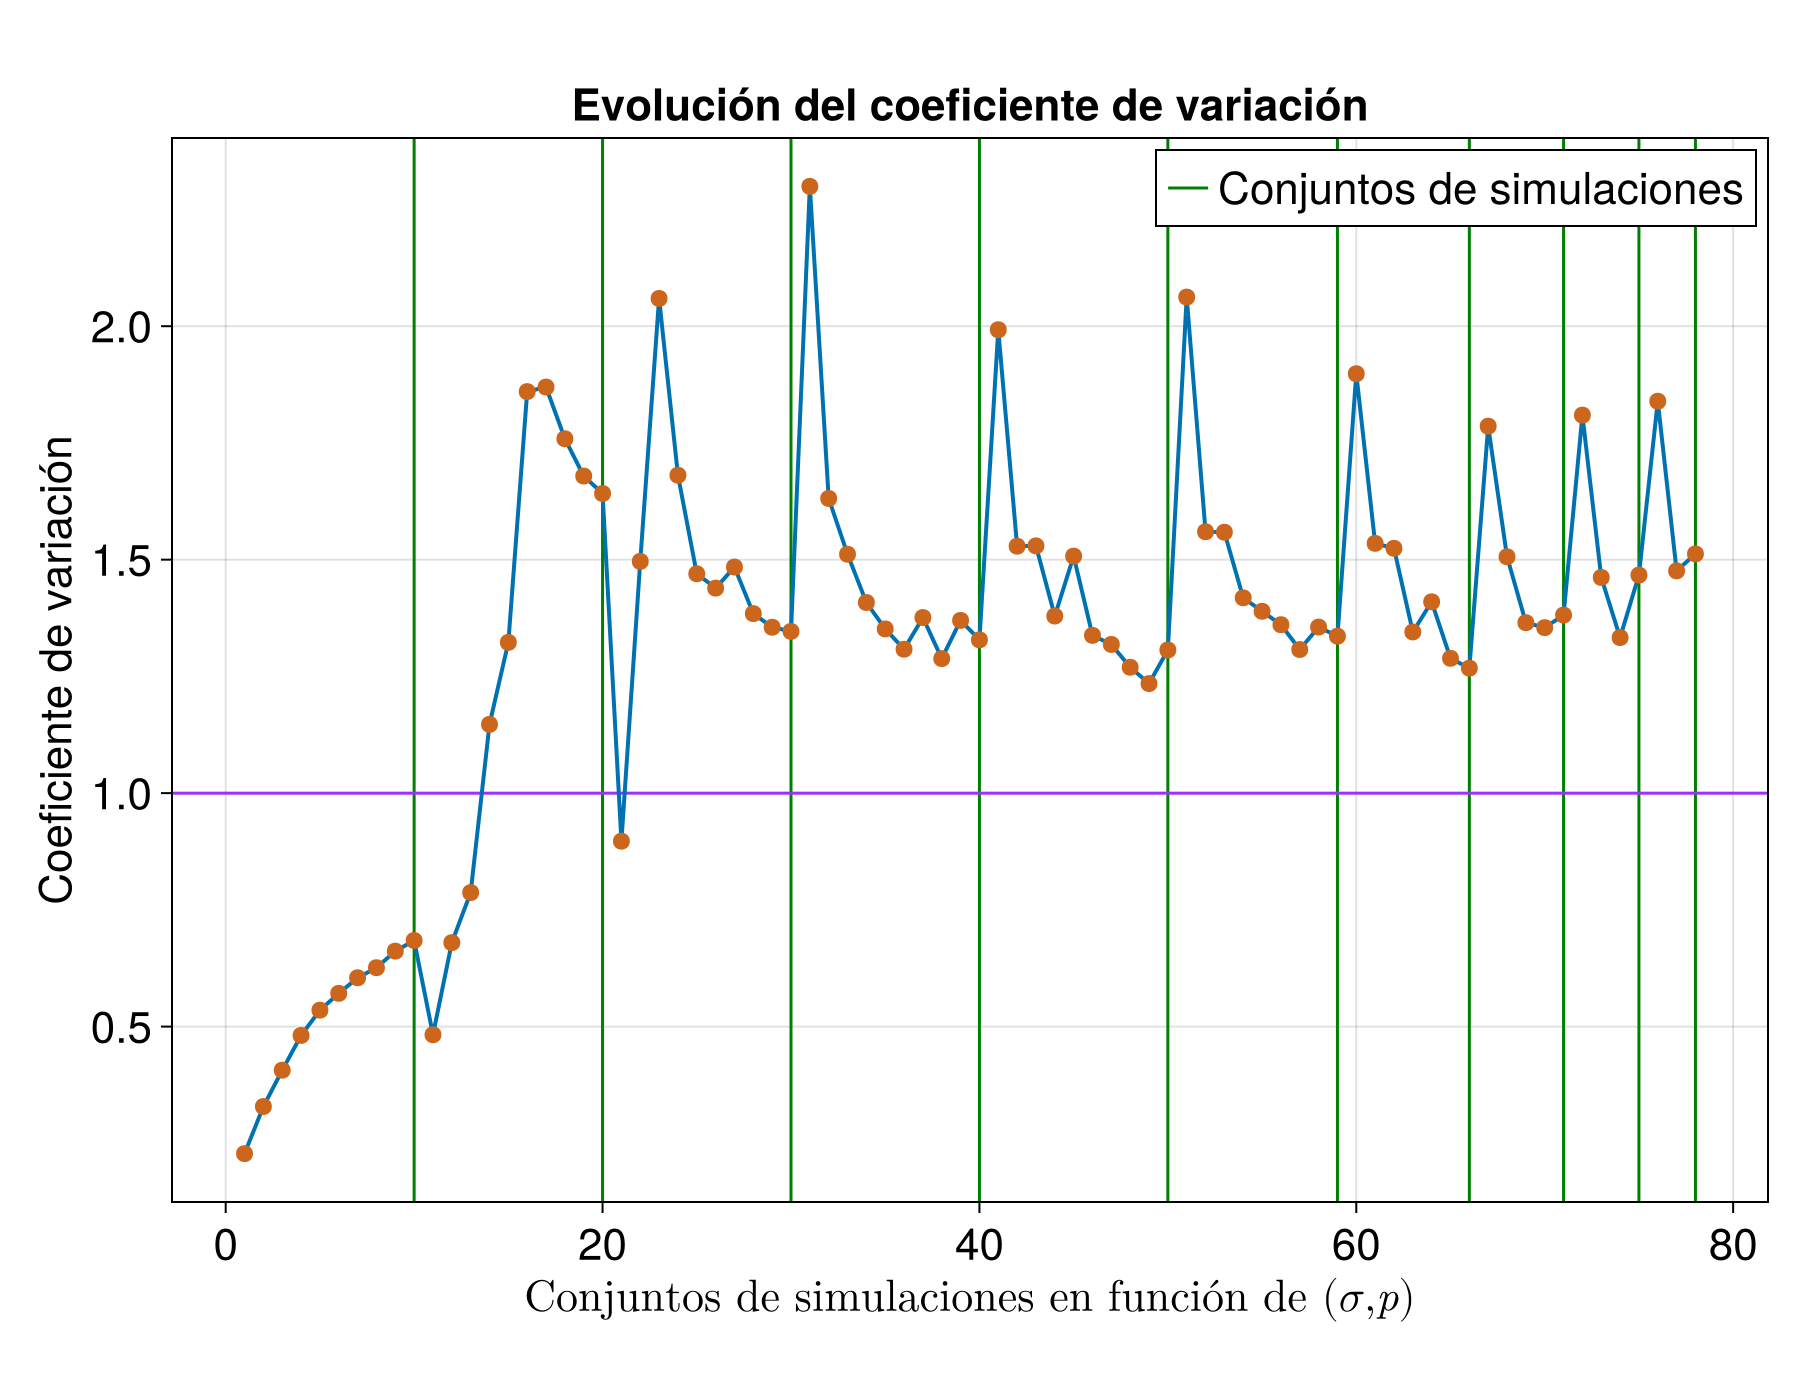
\includegraphics[scale=0.24]{../Imagenes/CoeficientesVariacion}
	\caption{Evolución del coeficiente de vaiación en función de $\sigma$ y $p$. Cada coeficiente se muestra para un conjunto de simulaciones dependientes de $\sigma_i$ y $p_j$ según la Tabla (\ref{tab:Simulaciones}).}
	\label{fig:CoeficientesVariacion}
\end{figure}

Del gráfico se pueden analizar varios puntos: para el conjunto de datos $\sigma=0.1$ se observa que la desviación estándar es menor al valor de sus medias, lo que indica que no son distribuciones muy dispersas o de cola pesada tal y como sucede con el resto de las distribuciones, además de que se ha observado que se comienza en una FDP normal que se va sesgando hacia la izquierda conforme $p$ aumenta. Esto se puede apreciar desde el esbozo de la Figura (\ref{fig:distDiagonales50}). Además del sesgo, si se encuentra bien marcada la tendencia de que la dispersión aumente conforme $p$ también lo haga. Ocurre algo interesante para $\sigma=0.2$, comienza con baja dispersión con respecto de la media y para $p\geq0.4$ emergen las distribuciones con alta dispersión. En este caso también se observa una ligera transición entre una FDP normal truncada que se va sesgando hacia la izquierda, sin embargo el resto de conjuntos de $\sigma$ las distribuciones comienzan sesgadas hacia la izquierda con cola pesada.\\
\\
A partir de $\sigma=0.3$ en adelante se puede observar un patrón interesante, se tiene un punto máximo del coeficiente de variación que indica una máxima dispersión y después disminuye, como si la cola pesada se suavizara. Y justamente eso es lo que ocurre, para cada $\sigma\geq 0.3$ con $p=0.1$, un gran porcentaje de la distribución se concentra cerca de la media mientras que son muy pocos los valores que se encuentran en la cola pesada. Conforme $p$ vaya aumentando en estos escenarios, la desviación estándar va disminuyendo con respecto de la media lo que indica que la distribución es cada vez menos dispersa haciendo que a su vez existan más valores que se concentren en la cola pesada. ¡Y esto ocurre similarmente para cada $\sigma\geq 3$!\\
\\
Algo importante de preguntarse es ¿por qué en general las distribuciones son de cola pesada con sesgo negativo? todo viene a raíz de como se definió la matriz de interacciones (Definición \ref{def:MatrizInteracciones}) y a su vez de como está construida la matriz de incidencias (Definición \ref{def:MatrizIncidencias}). Es fácil responder la parte del signo, desde un principio las diagonales siempre fueron negativas y se encuentra sustentado en la Proposición \ref{prop:DiagonalI}, por lo que las distribuciones siempre tuvieron que ser negativas\footnote{Aunque si se observa en la \ref{fig:distDiagonales50} se puede ver como para $\sigma$ y $p$ altas, las distribuciones tienen valores positivos; esto podría no ser congruente con la Proposición \ref{prop:DiagonalI} y más adelante se discutirá lo que ocurrió aquí.} pero con el carácter de cola pesada y además sesgada se tendrá que desarrollar un argumento más fuerte.\\
\\
Aunque estas distribuciones no tengan relación con FDP Log-Normales, es posible rescatar algunos elementos de su construcción para argumentar nuestra conjetura actual. Es bien conocido que para una variable aleatoria: si sus cambios son multiplicativos entonces se genera una distribución de cola pesada [cita\footnote{Para una variable aleatoria $X$, si el proceso multiplicativo es $X_t=X_{t-1}\cdot e	^{\epsilon_t}$, donde $\epsilon_t\sim \mathcal{N}(\mu,\sigma^2)$.}]. Además de ello, los mismos factores multiplicativos son los que determinan el sesgo de la distribución, en nuestro caso particular: de carácter negativo. Recordar que los valores de la diagonal vienen determinados por

$$\mathcal{I}_{ii} = r_i \left (1-\frac{2x_i+\sum_{j\neq i}\alpha_{ij}x_j}{K_i}\right ),\qquad\text{para }i\in\{1,...,N\}$$
\newpage
Claramente el término de la tasa de crecimiento $r_i$ reescala a todo $\mathcal{I}_{ii}$ de modo que las fluctuaciones que se generen con base en $x_i$ y $x_j$ se magnifican en función de esta $r_i$. No obstante, el valor intrínseco del término de la diagonal viene bien dictada por la relación de estas $x_i$ y $\alpha_{ij}x_j$ divididos por $K_i$\footnote{Donde las $x_j$ y $x_i$ son las entradas del atractor del sistema.}, donde se sabe que estos coeficientes vienen de una distribución normal centrada en $\mu=0$ con las $\sigma$s que se han venido considerando hasta ahora. Por lo tanto bien pueden existir valores extremos que se ubiquen en la cola pesada como puede haber valores que se concentren entorno a una media ($\langle d_{kk}(\sigma_i,p_j)\rangle$, Ver Figura (\ref{fig:TrMedStd}, \textbf{B})) dependiendo totalmente de como se encuentren configuradas las $\alpha_{ij}x_j$ que como recordatorio: vienen de la \textit{red de incidencias}. \\
\\
El motivo del sesgo se deberá a que son más comunes los coeficientes de interacción $\alpha_{ij}$ de la distribución normal entorno a $\mu=0$ con su respectiva $\sigma$ en comparación con los que se encuentren en los extremos de la misma, en especial cuando se tienen pocas interacciones ($p$ baja). Por lo tanto las sumas y el re-escalamiento de $\mathcal{I}_{ii}$ se concentra entorno a cierta moda estadística y en concreto	se ajusta en torno a $2$ que coincide con el valor fijo que se le dio al parámetro $r_i$. Cuando se tienen mayor número de 
\begin{wrapfigure}{l}{0.5 \textwidth} \vspace{-30pt} \begin{center}
		\includegraphics[scale=0.135]{../Imagenes/ModasEstadísticas}
	\end{center}
	\vspace{-20pt} 
	\caption{Modas de las distribuciones de diagonales disponibles dadas por la Tabla (\ref{tab:Simulaciones}).}
	\vspace{-10pt}
	\label{fig:ModasEstadísticas}
\end{wrapfigure}
interacciones ($p$ alta) es más probable que aumente la cantidad de valores extremos de las $\alpha_{ij}$ asociadas a $\mathcal{N}(\mu=0,\sigma)$ y en consecuencia la suma y los reescalamientos pueden situarse en valores más allá del 2 tal y como se puede apreciar en la Figura (\ref{fig:ModasEstadísticas}). Esta causa es la clave para que la media $\langle d_{kk}(\sigma_i,p_j)\rangle$, la desviación estándar $s(\sigma_i,p_j)$ y la moda estadística de las distribuciones de valores de las diagonales de los sistemas \textbf{estables} se vaya desplazando cada vez más hacia los valores negativos conforme $\sigma$ y $p$ aumenten: la estructura multiplicativa subyacente de la diagonal de la matriz de interacciones y las fluctuaciones que producen $x_i$ en conjunto con las $\alpha_{ij}x_j$ divididos por $K_i$ son la causa de este comportamiento. Para verificar si verdaderamente se trata de una propiedad de los sistemas estables, se habrían de generar más experimentos para otras $r_i$ y $K_i$ y validar si es reproducible este comportamiento. 

\subsubsection*{Relación con la estabilidad y eigenvalores de los sistemas.}

¿Qué relación tienen las diagonales con la estabilidad del sistema? Una fuerte hipótesis se puede realizar a partir de ello, pues resulta que de todos los sistemas que resultaron estables (salvo unas excepciones), tienen a sus diagonales con sus elementos negativos, sugiriendo que la diagonal es una fuerte componente decisiva para volver a los sistemas estables. No existe por ahora un teorema que resuelva esta conjetura, pues deben existir contra ejemplos en donde los elementos de la diagonales son negativos pero el resto de entradas de la matriz impacta de tal modo que vuelve al sistema inestable. Por ahora las simulaciones sustentan el argumento de la estabilidad pero entonces ¿qué pasa con las diagonales que resultaron positivas?  respectivamente) ¿impactarán también en la distribución de eigenvalores con algunos de ellos con parte real positiva? ¿Con base en el procedimiento, como es que se llegó a estos escenarios? (Ver Figura (\ref{fig:distDiagonales50}) para $\sigma=\{0.4,0.7\}$ con $p=\{1.0,0.7\}$)\\
\\
Como el mecanismo para determinar que los sistemas fueran estables o no se hizo a partir de revisar que las series de tiempo no divergieran, ha sucedido que para $\sigma$ y $p$ cercanos a 1.0, los sistemas tienen mayor dificultad para estabilizarse por la cantidad de interacciones existentes, a su vez las fluctuaciones que se producen provocan el retardo  de la estabilización. Lo ideal hubiera sido prolongar el tiempo de integración a $t_f=100$ para estos casos y verificar si suceden dos cosas: o logran llegar al atractor o también es posible lleguen a un punto crítico inestable haciendo que divergan las soluciones tras un efecto de retardo igualmente. \\
\\
Por lo tanto, debido al tiempo de integración: las series de tiempo se han quedado a medias para resolver en alguno de los dos escenarios anteriores. Esto es importante ya que se ha tomado el último punto de la serie como aquel vector $N$-dimensional considerado para evaluar en la matriz jacobiana que da origen a la matriz de interacciones. En conclusión existe un cierto número de matrices de interacción con esta situación y que por lo tanto no son estrictamente matrices de interacción, pues no  se encuentran evaluadas sobre un punto crítico. Sin embargo se ha intentado realizar una técnica para poder intentar llegar a ese posible atractor: consiste en utilizar el método de Newton-Rhapson multivariado para hallar el punto crítico que se espera.\\
\\
Se utilizaría como condición inicial el último punto de la serie de tiempo ya que se esperaría que el atractor estuviera cerca de esa región y se llegaron a dos resultados principales: Si la matriz resultante tiene de 1 a 3 entradas positivas, es probable que si encuentre el atractor y entonces terminemos de concluir que si se trataba de un sistema estable. El segundo resultado es menos esperanzador, pues si se tienen más de 3 entradas positivas, aún ejecutando Newton-Rhapson multivariado con las condiciones mencionadas, el algoritmo no devuelve al punto crítico atractor: de aquí se desprenden dos posibles escenarios, el primero y más directo es simplemente asumir que el sistema no era estable y que tuvo una acción retardada para que las soluciones divergieran. El segundo escenario es que debido a la condición inicial propuesta, el algoritmo solamente pudo aproximarse a un punto silla que se encontraba más próximo que el atractor y que gracias a ello no sea posible acceder a este segundo punto crítico que es el que se espera.\\
\\
No es trivial encontrar puntos críticos para sistemas $N\gg1$ aún teniendo métodos numéricos que ayuden a simplificar la tarea, pues se sabe que existen más de $N$ en cuestión y no se sabe con exactitud en que región del hiper-espacio se encuentra al menos uno de ellos que es el atractor. Por lo que se concluye esta parte con el hecho de que no hay forma de saber con la información actual que tipo de estabilidad tenían, la alternativa sería repetir esos experimentos considerando un tiempo de integración mayor a $50$ esperando que lleguen a su respectivo atractor.\\
\\
Excluyendo por ahora los casos de las diagonales con entradas positivas, ¿cual es la relación de las diagonales negativas con respecto de la estabilidad de los sistemas? Se puede plantear que mientras las trazas de las matrices sean negativas el sistema es estable, pero en esto hay que poner una restricción: las trazas negativas con todos lo valores de la diagonal negativos. Si existe al menos un valor positivo en la diagonal del Jacobiano del sistema, entonces cabe la posibilidad de que exista al menos un eigenvalor positivo que volvería intestable al sistema. Los experimentos han mostrado que la diagonal es un factor determinante para la estabilidad de estos sistemas, aunque no es absoluto si es un requisito importante que debe cumplirse. Las trazas de las matrices guardan una íntima relación con las medias ($d_{kk}(\langle \sigma_i,p_j)\rangle$) y a su vez como ya se ha visto anteriormente, con la desviación estándar $s(\sigma_i,p_j)$
\begin{figure}[h!]
	\centering
	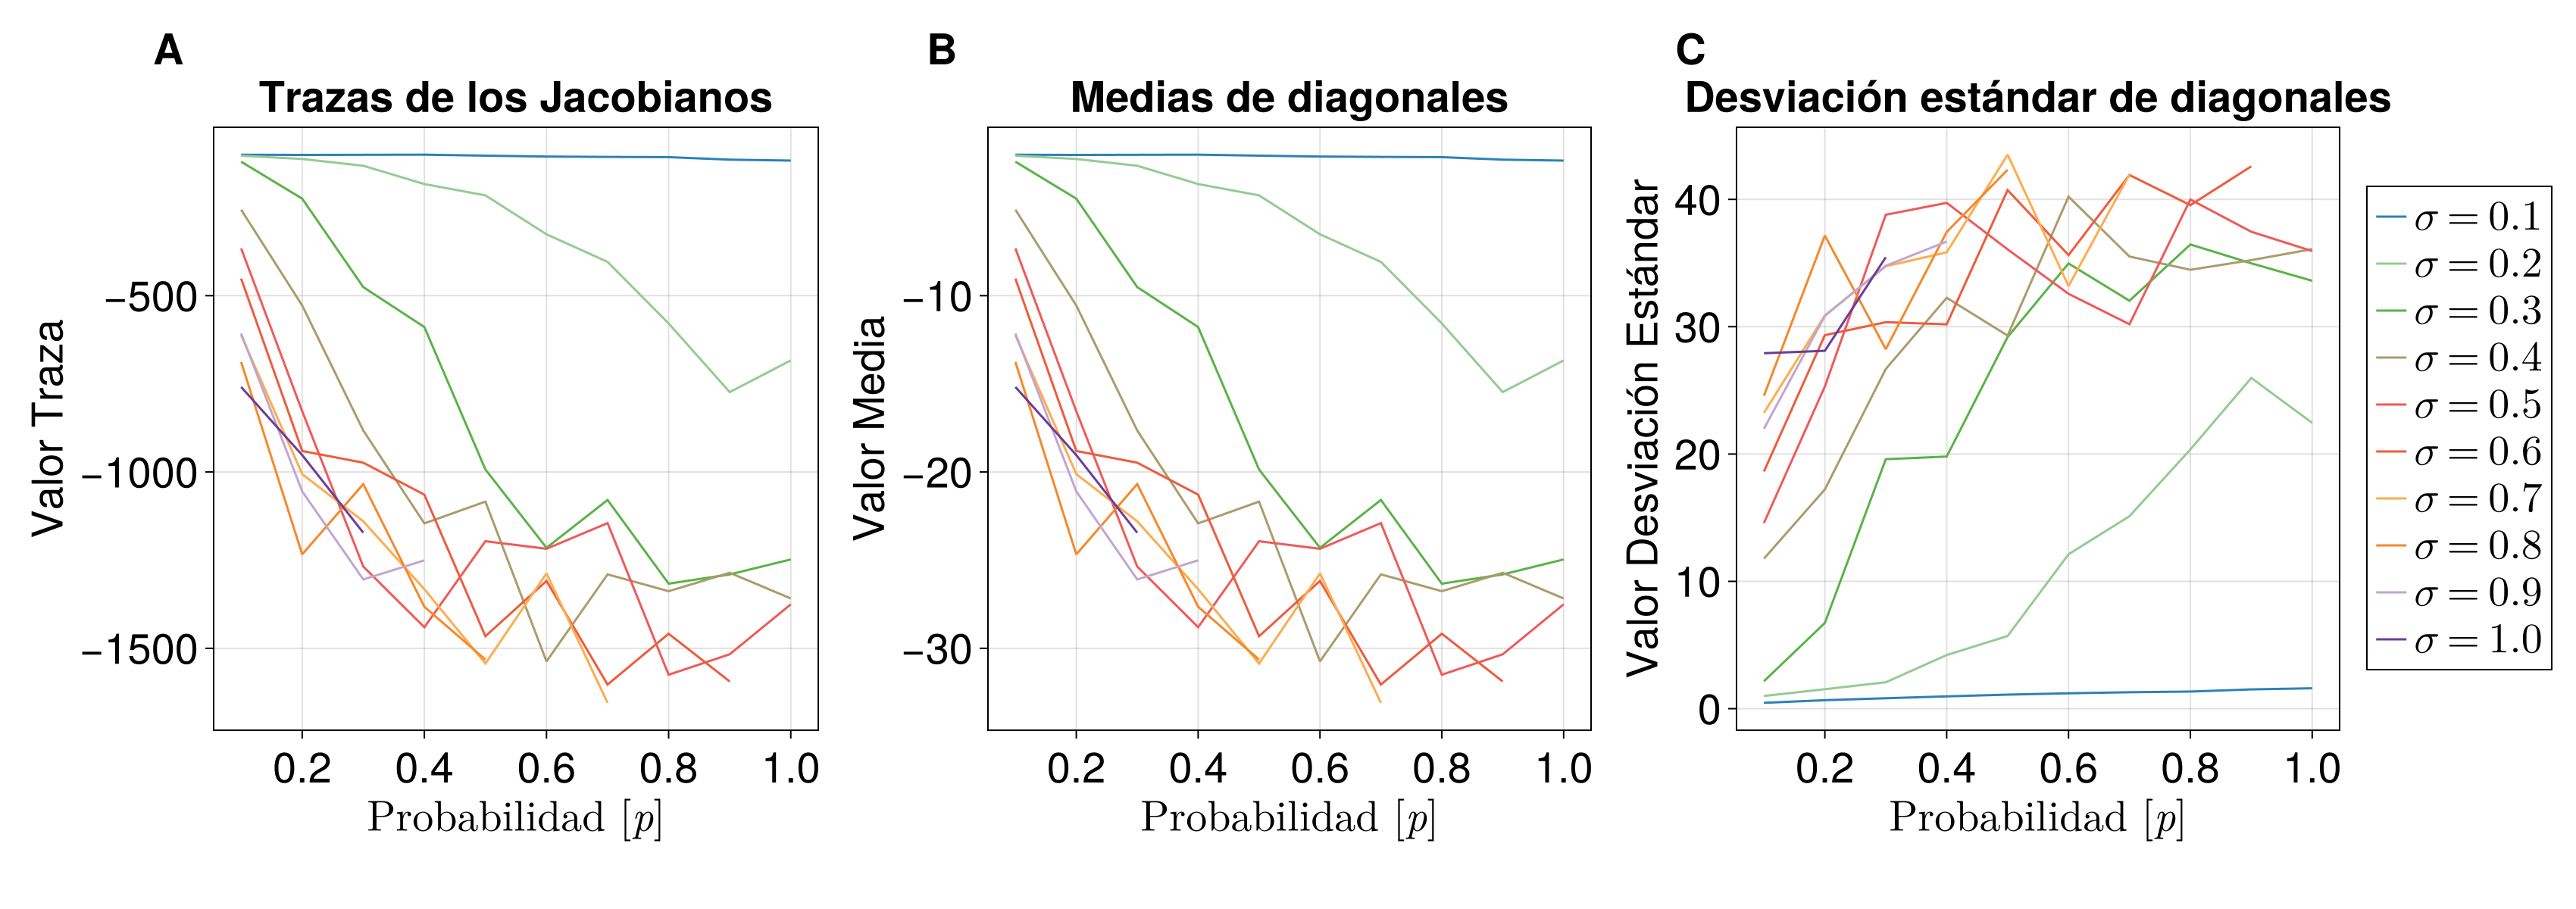
\includegraphics[scale=0.15]{../Imagenes/TrMedStd}
	\caption{Cada una de las cantidades se considera con base en las simulaciones disponibles. (\textbf{A}) Evolución de las trazas de los jacobianos del sistema. (\textbf{B}) Evolución de las medias de las diagonales de los jacobianos del sistema. (\textbf{C}) Evolución de la desviación estándar de las diagonales de los jacobianos del sistema.}
	\label{fig:TrMedStd}
\end{figure}

Aquí se puede ver de manera directa la relación que aparece retratada en la Figura (\ref{fig:CorrelacionMvsStd}), a medida que la traza/media de las simulaciones disminuye hacia valores cada vez más negativos, la desviación estándar por el contrario va aumentando. ¿Cuál será la relación de las diagonales de los jacobianos con respecto de su distribución de eigenvalores?

\subsubsection*{Distribución de valores propios}

Anteriormente se había propuesto, con un argumento cualitativo de la Figura (\ref{fig:LeyesCirculares}), que existen $N$ \textit{leyes circulares} donde a cada una de ellas le corresponde un centro y radio de cada valor de la diagonal del jacobiano del sistema. De esta manera cada ley circular encierra cierta cantidad de valores propios del sistema. Con la información provista de las simulaciones realizadas, se puede determinar un argumento estadístico más fuerte para sostener esta propuesta. \\
\\
La clave estará en revisar si existe una correlación estadística entre los valores de las diagonales mencionadas con las partes reales de los eigenvalores, se ha observado que para algunas simulaciones la relación fue casi perfecta mientras que para otras no tanto. Lo interesante de ver es que la relación es mejor cuando el valor de $p$ es alto, es decir, cuando hay cada vez más interacciones y para cuando las distribuciones de las diagonales son menos dispersas. Tomando una simulación al azar, se aprecia la siguiente relación entre partes reales de los eigenvalores con las diagonales de los jacobianos calculados
\begin{figure}[h!]
	\centering
	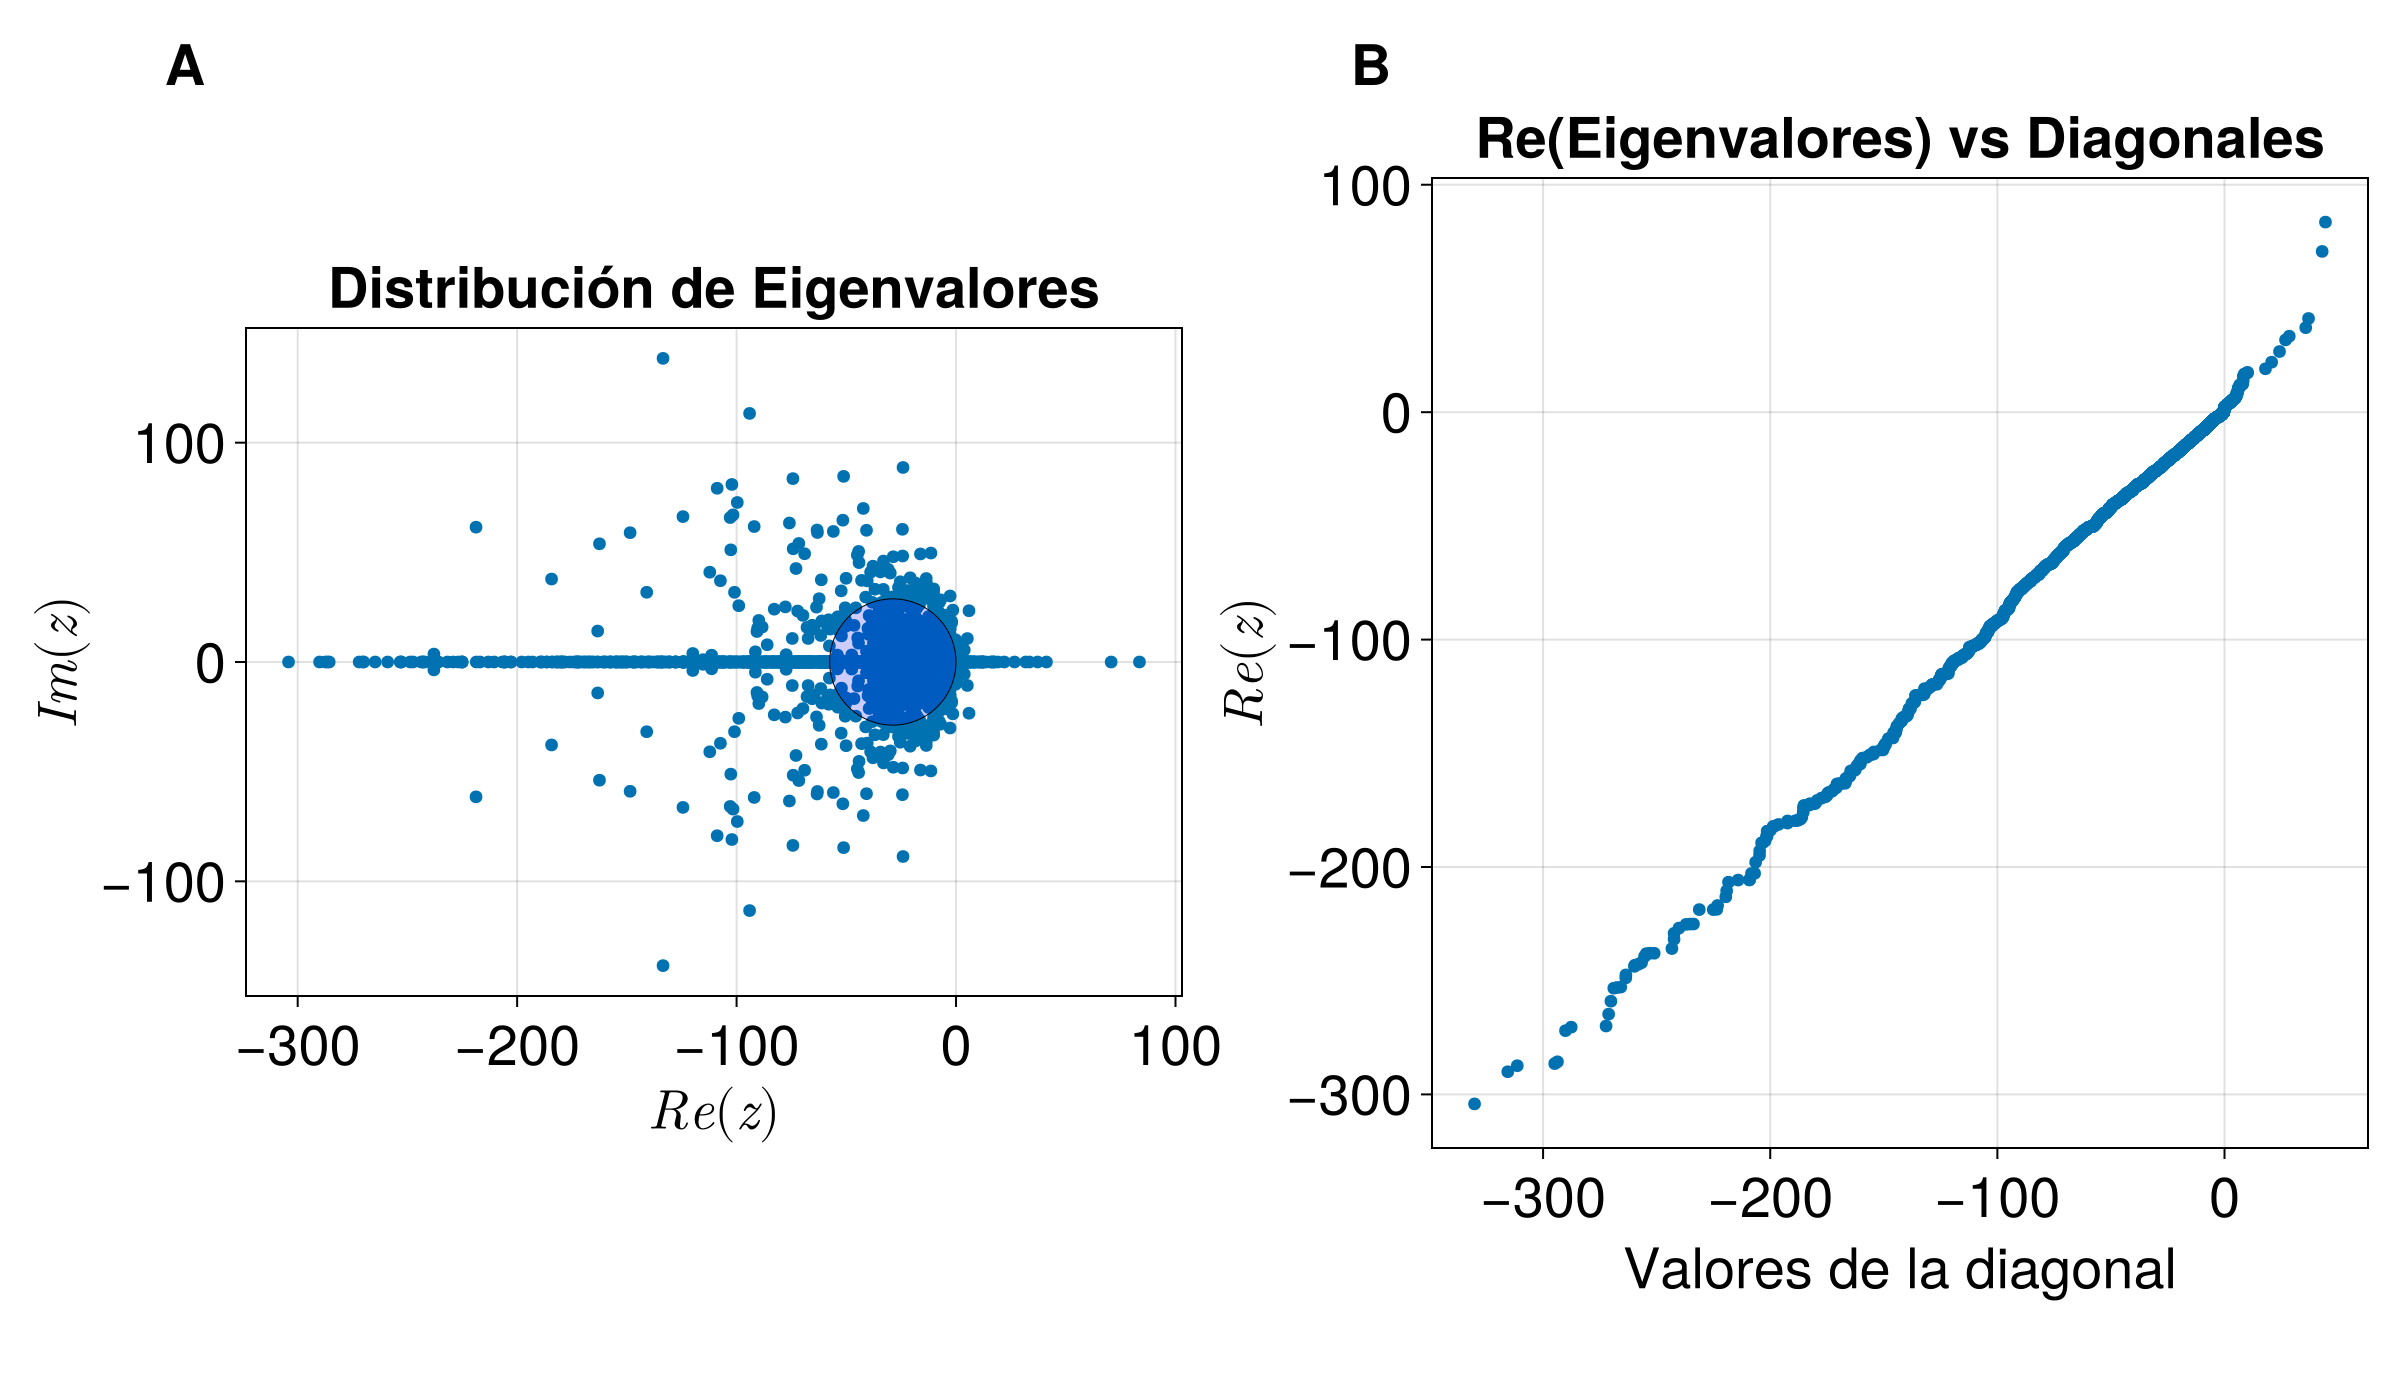
\includegraphics[scale=0.2]{../Imagenes/ReEvs-Diagonales}
	\caption{(\textbf{A}) Distribución de valores propios de 100 jacobianos para el caso $\sigma=0.5$, $p=0.4$. Se agrega una ley circular correspondiente al valor medio de la distribución de diagonales. (\textbf{B}) Relación entre la parte real de los valores propios con las diagonales de los jacobianos considerados.}
	\label{fig:ReEvs-Diagonales}
\end{figure}

En la distribución de valores propios hay algunas características a analizar: Se ha agregado una ley circular con centro y radio correspondiente al valor medio de su distribución de valores; encierra una gran cantidad de valores propios concentrados en la mancha. Por otro lado se observan valores propios positivos, esto deviene de la discusión que anteriormente se tuvo con respecto de las entradas positivas de las diagonales de los Jacobianos. Hay un porcentaje de éstos que tuvieron valores propios positivos, para evitarlos se debe de considerar en futuras simulaciones un tiempo de integración mayor a 50. En cuanto a la relación entre partes reales de valores propios y elementos de la diagonal de los Jacobianos considerados, existe una relación lineal casi perfecta para el caso particular: $\sigma=0.5$ y $p=0.4$. Sobre todo es interesante ver que incluso existe una relación entre las entradas positivas de las diagonales con los valores propios con parte real positiva, esto ya habla más de la estructura del Jacobiano. En otras distribuciones el ajuste puede ir variando pero en general se sigue esta tendencia entre ambos valores considerados.\\
\\
Para explorar más a profundidad sobre el panorama completo de las simulaciones, se verá la relación entre la media, mediana y moda de las diagonales con respecto de las partes reales de los valores propios de cada uno de los 78 conjuntos de simulaciones; con ello se verá si es que realmente existe una relación lineal entre estas cantidades. Sin embargo, aunque estos sean valores representativos de cada una de las distribuciones, sigue siendo esbozo general.
\begin{figure}[h!]
	\centering
	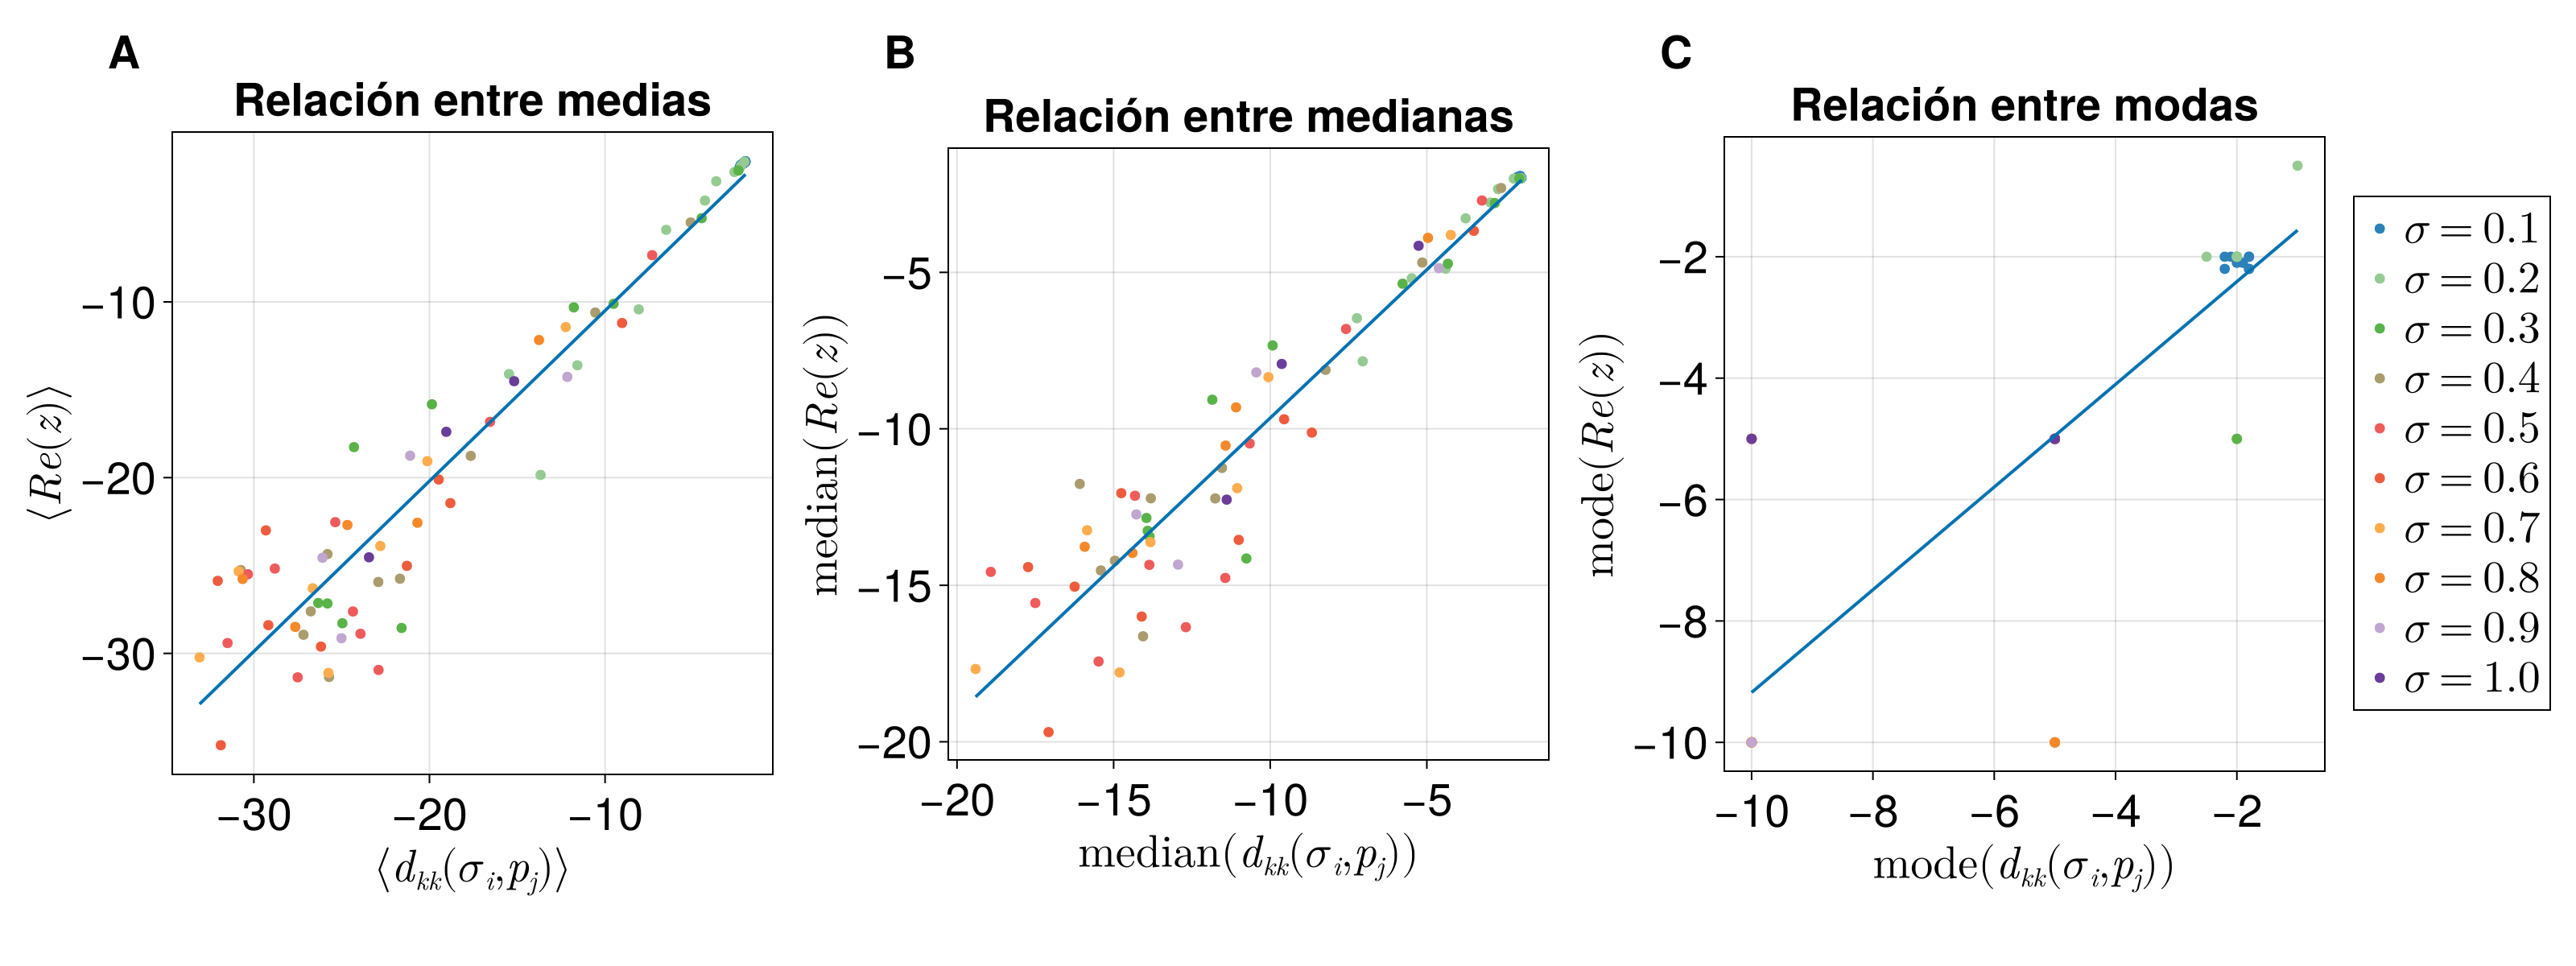
\includegraphics[scale=0.16]{../Imagenes/AjustesLinMeds}
	\caption{(\textbf{A}) Ajuste lineal de la relación entre las medias de las $Re(\overline{\lambda})$ con las medias de las $d_{kk}(\sigma_i,p_j)$ de los Jacobianos del sistema. (\textbf{B}) Ajuste lineal de la relación entre las medianas $Re(\overline{\lambda})$ con las medianas de las $d_{kk}(\sigma_i,p_j))$ de los Jacobianos del sistema. (\textbf{C}) Ajuste lineal de la relación entre las modas de $Re(\overline{\lambda})$ con las modas de las $d_{kk}(\sigma_i,p_j)$ de los Jacobianos del sistema.}
	\label{fig:AjustesLinMeds}
\end{figure}

Estos ajustes lineales al igual que en la Figura (\ref{fig:CorrelacionMvsStd}) es un ajuste general sobre los 78 conjuntos, lo ideal sería realizar un ajuste lineal para cada conjunto $\sigma_i$. Pero de estos gráficos se puede apreciar que para valores cercanos a cero, los 3 casos se ajustan a la recta. Lo que indica que la correlación entre las $d_{kk}(\sigma_i,p_j)$ y las $Re(\overline{\lambda})$ es compartida para toda $\sigma$ con una baja probabilidad de conectividad. Conforme esta $p$ vaya aumentando, entonces la relación lineal se vuelve específica tal y como se mencionó anteriormente. Esta relación esta sugiriendo que la distribución de $Re(\overline{\lambda})$ es semejante a las distribuciones de $d_{kk}(\sigma_i,p_j)$, es decir, ¡de cola pesada y con sesgo negativo! Sin embargo como se mencionó antes: estas medidas aunque son representativas no muestran el panorama completo como en la Figura (\ref{fig:ReEvs-Diagonales} \textbf{B}), pues solo se esta considerando la relación lineal de 3 casos particulares representativos de las distribuciones consideradas. 
\begin{figure}[h!]
	\centering
	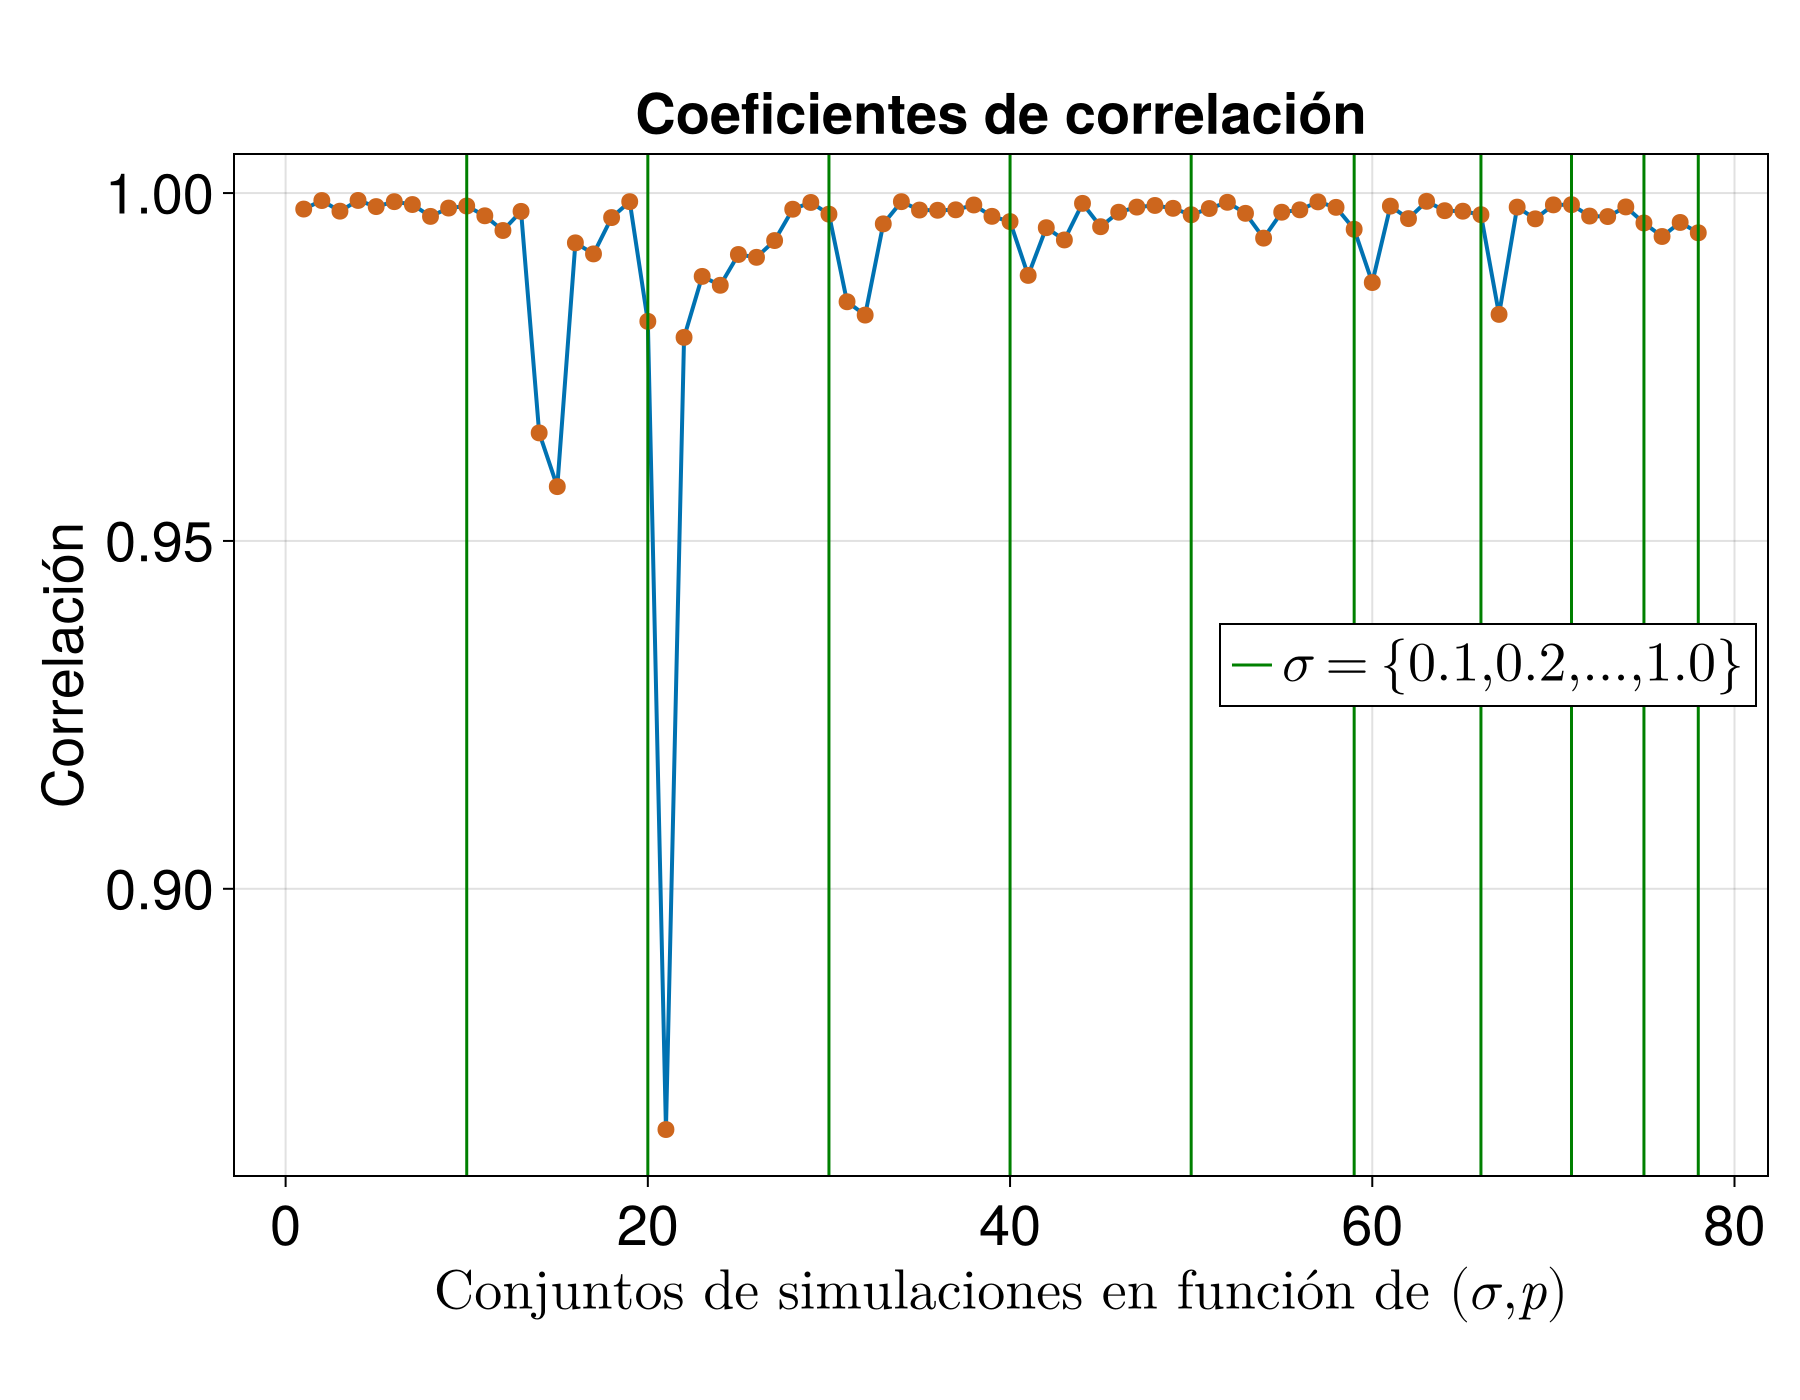
\includegraphics[scale=0.2]{../Imagenes/CoeficientesCorrelacion}
	\caption{Coeficientes de correlación en función de $\sigma$ y $p$. Cada coeficiente corresponde para un conjunto $\sigma_i$ y $p_i$ de simulaciones según la Tabla (\ref{tab:Simulaciones}).}
	\label{fig:CoeficientesCorrelacion}
\end{figure}

Al igual que como se hizo para el coeficiente de variación en la Figura (\ref{fig:CoeficientesVariacion}), se puede armar un mapa de coeficientes de correlación para cada conjunto de simulaciones, de esta manera se podrá ver que tan fuerte o débil es la relación entre $Re(\overline{\lambda})$ y $d_{kk}(\sigma_i,\sigma_j)$. Se puede apreciar que la correlación es sumamente 
\begin{wrapfigure}{r}{0.5 \textwidth} \vspace{-30pt} \begin{center}
		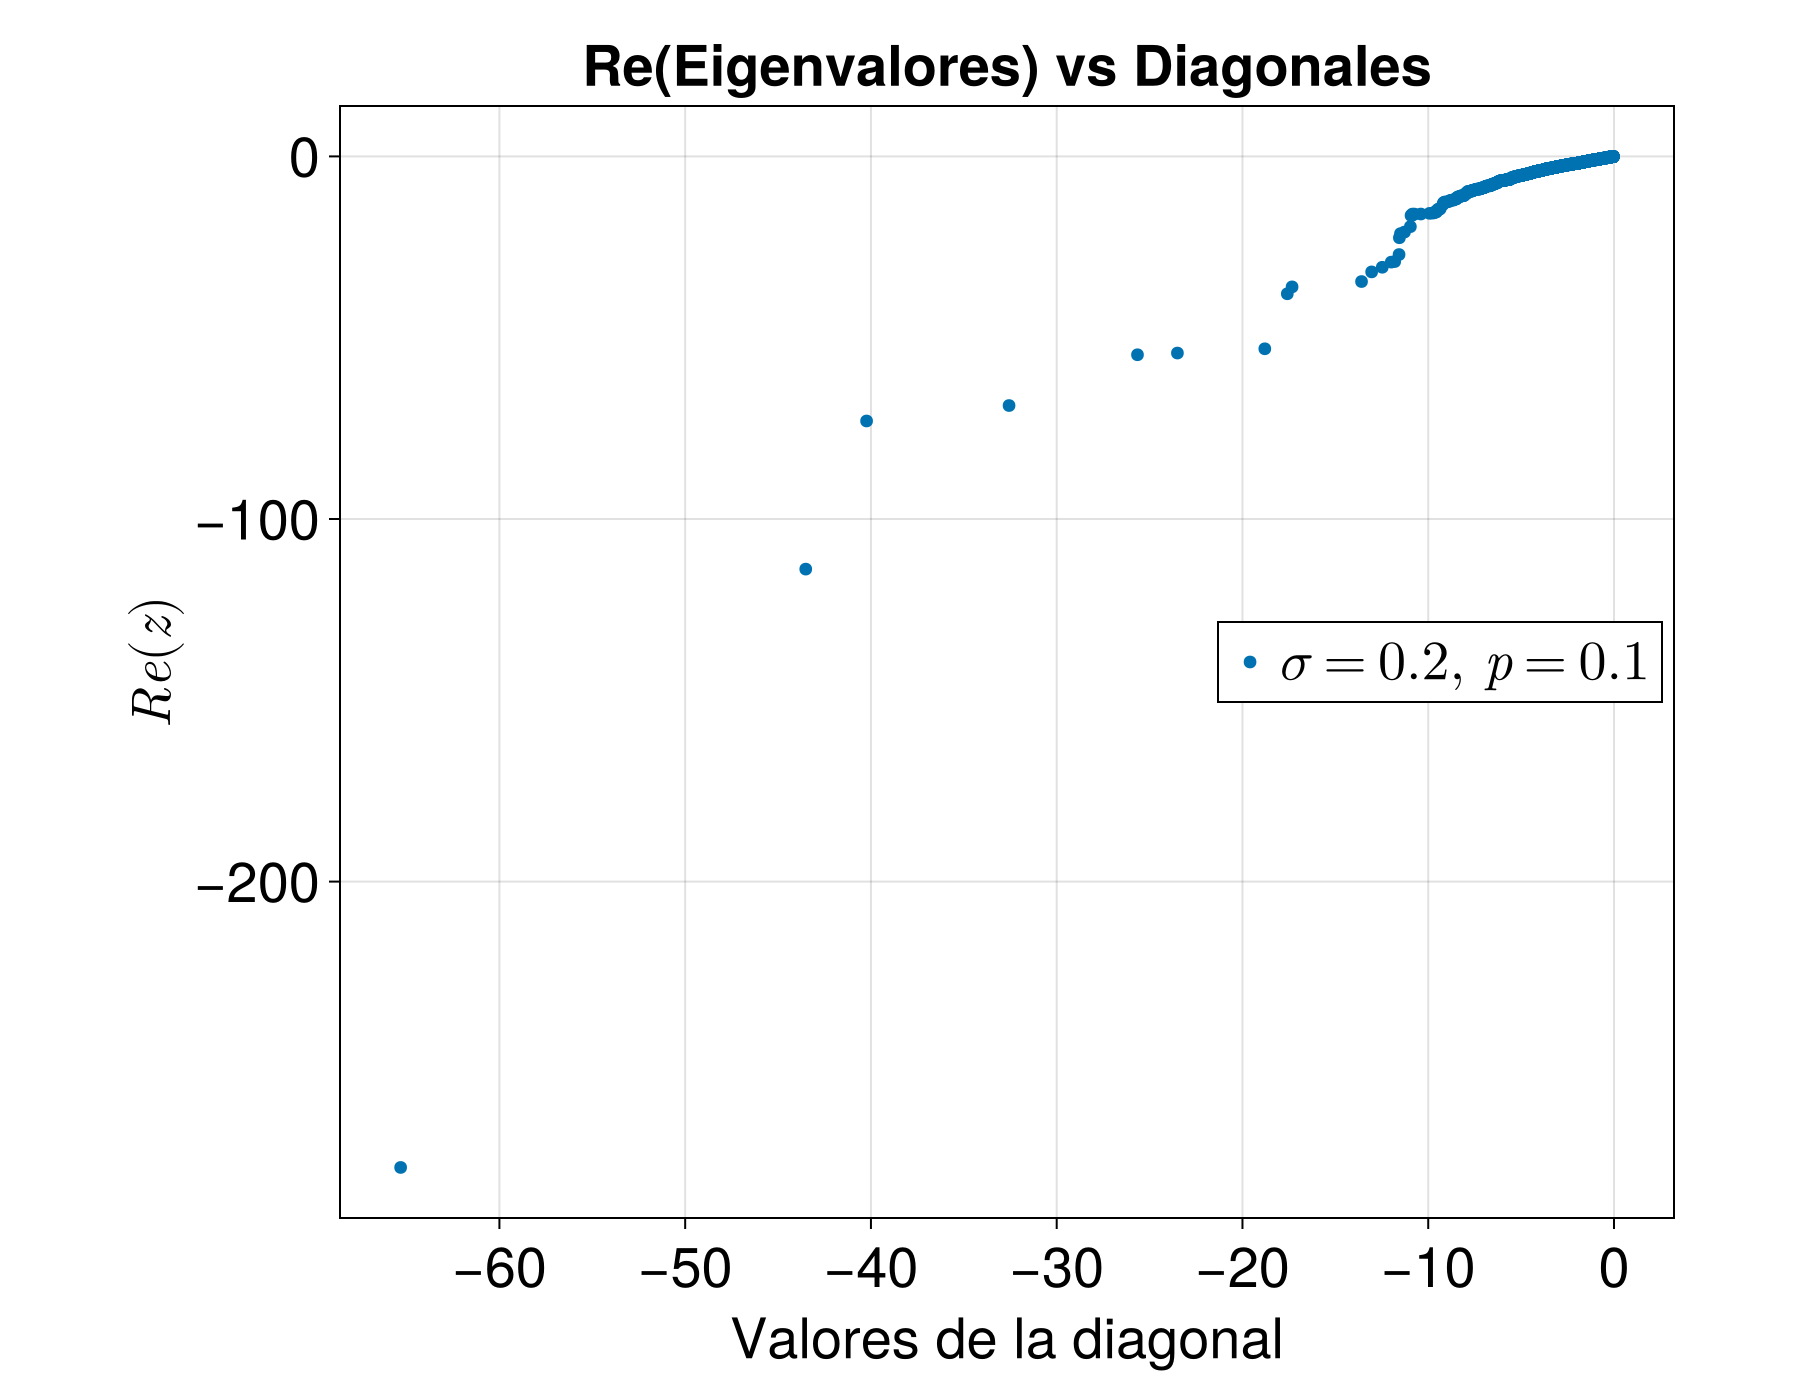
\includegraphics[scale=0.135]{../Imagenes/AnomaliaSim21}
	\end{center}
	\vspace{-20pt} 
	\caption{Anomalía de la simulación 21, caso con $\sigma=0.3$ y $p=0.1$.}
	\vspace{-10pt}
	\label{fig:AnomaliaSim21}
\end{wrapfigure}
fuerte para la gran mayoría de los casos, con valores superiores a $0.98$ lo que indica que las distribuciones de $d_{kk}(\sigma_i,p_j)$ y de $Re(\overline{\lambda})$ no son solamente semejantes sino prácticamente iguales o con muy poca variación. Solamente se tiene una anomalía para el caso $\sigma=0.3$ y $p=0.1$ en el que su coeficiente de correlación es abruptamente más bajo que el resto del conjunto de simulaciones. Viendo como es la relación de este caso particular se observa si hay una tendencia lineal pero hay valores anómalos que no tienen relación entre sí, pues incluso difieren por un orden de magnitud. Sin embargo la tendencia es clara a pesar de las anomalías, el coeficiente es próximo a $0.8654$ y sigue marcando una fuerte correlación entre $Re(\overline{\lambda})$ y $d_{kk}(\sigma_i,p_j)$. Por lo tanto bajo este análisis se puede justificar la propuesta de las $N$ leyes circulares de la Figura (\ref{fig:LeyesCirculares}), los elementos de la diagonal están profundamente relacionados con la distribución de valores propios en el plano complejo. Cada elemento de la diagonal puede ser visto como centro y radio de una ley circular particular y que será capaz de encerrar cierto porcentaje de valores propios que se encuentren a su alcance y dentro de su vecindad.\\
\\
Para concluir esta sección se tienen algunos puntos a abordar; en primer lugar se debe de ver que los casos presentados en esta sección son particulares para $N=50$, habría de definir otros tamaños de matrices para verificar si se siguen los patrones descritos anteriormente. Pero para el mismo caso de $N=50$ se deben de probar más experimentos para otros tipos de tasas de crecimiento y de capacidades de carga, diferentes de $r=2$ y $K=5$ e incluso probar para distribuciones de $r_i$ y de $K_i$ pero claro que al hacerlo se le puede subir uno o varios niveles de complejidad al problema. Al hacer esto se podrá ver si verdaderamente la estructura que se vio en esta sección es universal para cualquier parámetro que se maneje.\\
\\
Los resultados principales de esta sección se enumeran a continuación, las distribuciones de elementos de la diagonal de los Jacobianos asociados al sistema de Lotka-Volterra generalizado siguen una tendencia de distribución de cola pesada con sesgo negativo. Estas distribuciones guardan una relación entre la media y la desviación estándar de modo que para toda $\sigma$, mientras la $p$ aumenta, se ve como la media se recorre hacia valores negativos mientras que la desviación estándar va aumentando. En esta dirección se pudo apreciar que para $\sigma\geq 0.3$ con $p$ bajas: el coeficiente de variación es más grande lo que indica que existe una mayor dispersión en estas distribuciones que en aquellas con $\sigma\geq 0.3$ y $p$ altas, en donde se tienen cada vez más valores en la cola pesada.\\
\\
Las trazas son determinantes para definir la estabilidad del sistema pero no es un criterio absoluto, si se tienen elementos positivos en la diagonal el sistema puede presentar valores propios positivos lo que indica inestabilidad. La misma estructura del Jacobiano del sistema (\ref{eqn:MartizInteracciones}) garantiza los elementos de la diagonal negativos siempre y cuando se evalúe sobre un punto crítico atractor. Las simulaciones nos han confirmado que todo jacobiano evaluado en el atractor produce diagonales con elementos negativos. Por último se ha observado una fuerte correlación entre las $Re(\overline{\lambda})$ y las $d_{kk}(\sigma_i,p_j)$ de los jacobianos del sistema, lo que soporta la justificación de la propuesta de la $N$ leyes circulares que establece que cada uno de los elementos de la diagonal es un centro y radio de una determinada ley circular que encierra cierto porcentaje de valores propios. \\
\\
Además de las propuestas antes mencionadas para investigar otros escenarios del Jacobiano del sistema, una de las cosas que haría falta para completar este trabajo es ver como es la distribución de valores de los elementos fuera de la diagonal de los jacbianos del sistema, ver si son de cola pesada o si tienen algún tipo de sesgo. Observar, caracterizar y ajustar a una distribución conocida para poder crear una receta y así generar estas matrices sin la necesidad de pasar por todo los métodos antes descritos en esta tesis. Un pequeño adelanto de esta idea es comenzando por analizar las curtosis y las modas estadísticas de los elementos fuera de la diagonal de los Jacobianos de uno  de los 78 conjuntos de simulaciones únicamente para saber donde se encuentra el pico de la distribución y determinar si también son de cola pesada
\begin{figure}[h!]
	\centering
	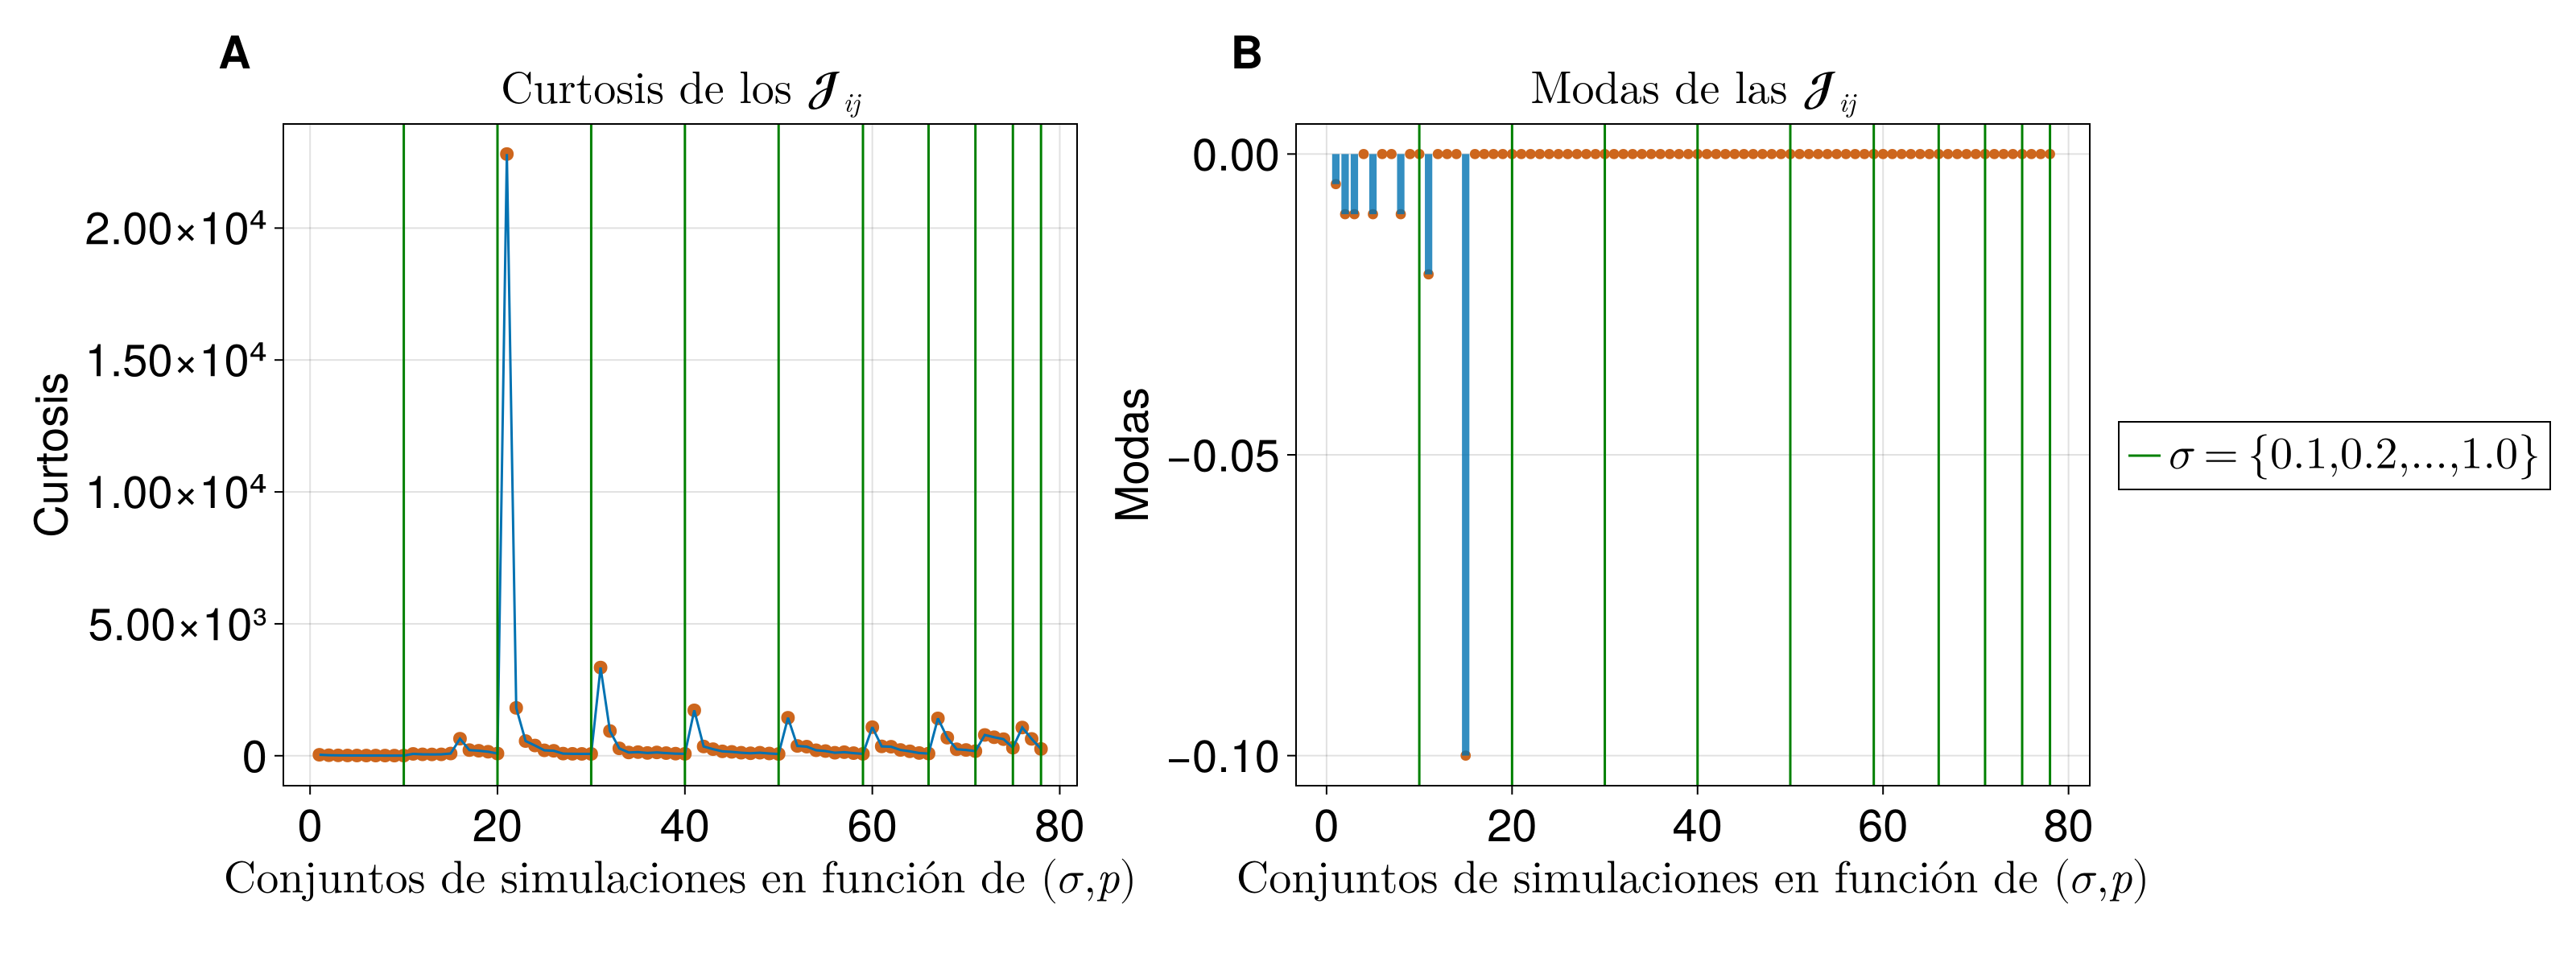
\includegraphics[scale=0.16]{../Imagenes/CurModasJij}
	\caption{(\textbf{A}) Coeficientes de curtosis de los elementos fuera de la diagonal de los Jacobianos del sistema. (\textbf{B}) Modas estadísticas de los elementos fuera de la diagonal de los Jacobianos del sistema.}
	\label{fig:CurModasJij}
\end{figure}

Como se puede observar, son distribuciones muy raras pues en general tienen curtosis muy grandes en particular una que es exageradamente grande con respecto del resto. El valor más frecuente del coeficiente de curtosis para los 78 conjuntos de simulaciones es de 78 lo que sigue siendo muy alto. Además los picos generalmente se encuentran alrededor del cero salvo algunas excepciones. Todo indica que la distribución de valores que conforman los Jacobianos del sistema de Lotka-Volterra generalizado para $N=50$ con $r=2$ y $K=5$ y para cada $\sigma$ y $p$ son sumamente raras: conformados por distribuciones de cola pesada con sesgo negativo para las diagonales, y por distribuciones de cola super pesada centradas en cero para el resto de elementos del Jacobiano. Por lo que realizar la receta de la que se habló anteriormente será una tarea compleja.
\newpage
\section{Transiciones de estabilidad}

Para darle seguimiento a los resultados de esta tesis, ésta sección se va a centrar en explorar cuales son las condiciones de la matriz de incidencias (en función de $\sigma$, $p$ y $N$) para que los Jacobianos resultantes muestren estabilidad o no. Recordando una de las conclusiones de May: un sistema será estable si la conectancia del sistema (dada por $p$) es débil mientras que la fuerza de las interacciones (dada por $\sigma$) es considerablemente alta; y ésto es válido en sentido opuesto, si dicha fuerza es baja entonces existe la oportunidad de que el sistema sea estable con una alta conectividad. \\
\\
Para ello se van a considerar tres tipos de sistemas, para $N=\{100,50,25\}$. Se pretende ver que tanto cambia la estabilidad con diferentes tamaños del sistema (\ref{eqn:LK}). La metodología que se va a aplicar para resolver este problema es la siguiente: Para cada $N$ se va a realizar exactamente lo mismo salvo algunas variaciones, primero se va a integrar el sistema fijando la fuerza de interacción en los siguientes valores $\tilde{\sigma}=\{0.1,0.2,...,1.0\}$ mientras que para las probabilidades de conectividad se va a considerar la siguiente partición del intervalo $[0,1]$ para cada $N$:
\begin{equation}\label{eqn:particionLin}
	p = \{x_i\, |\, x_i=i\cdot\Delta x, i=0,1,2,...,100\},\qquad\text{con }\Delta x=0.01
\end{equation}
Con esta configuración de valores se permitirá generar diagramas de transición de estabilidad para cada $N$ en función de $p$ considerando que es una partición equidistante. Hay otros dos diagramas de estabilidad que son de interés; siguiendo en función de la probabilidad de conectividad se define la siguiente partición sobre el intervalo $[0,1]$
\begin{equation}\label{eqn:particionLog}
	p_{\log}=\left \{ x_i\, |\, x_i=10^{-\left (10-\frac{10i}{99}\right )},\ i=0,1,...,99\right \}
\end{equation}
Se ha considerado particularmente este conjunto de probabilidades de conectividad ya que para ciertas $\sigma$ y para $N=100$ primordialmente, la transición ocurre de manera abrupta de tal modo que en la escala lineal no se aprecia cuando ocurre la transición, por ende se permite visualizar este cambio para valores muy pequeños. Más adelante se irá viendo este fenómeno. Por último pero no menos importante, se van a considerar diagramas en donde se deja fija la $p$ para cada $N$ y se define una partición equidistante en el intervalo $[0,1]$ en función de la fuerza de interacción, es decir:
\begin{equation}
	\sigma = \{x_i\, |\, x_i=i\cdot\Delta x, i=0,1,2,...,100\},\qquad\text{con }\Delta x=0.01
\end{equation}
Para esta configuración de valores se obtendrán los diagramas de transición en función de $\sigma$ y se verá que tan contrastante es con respecto de los otros diagramas de transición. Teniendo las particiones y los ajustes de parámetros necesarios para generar los diagramas de transición, solamente falta ver cómo y de qué manera se van a generar estos diagramas. Para cada $N$, $\sigma$ y $p$ con sus correspondientes particiones se va a integrar el sistema cierto número de veces por cada elemento de ésta misma:
\newpage
\begin{table}[h!]
	\centering
	\begin{tabular}{|c|c|}
		\hline
		Tamaño del sistema $N$ & Cantidad de simulaciones por cada elemento de la partición  \\ \hline
		100 & 3000 \\ \hline
		50  & 6000 \\ \hline
		25  & 12000 \\ \hline		
 	\end{tabular}
	\caption{Cantidad de simulaciones realizadas por cada $N$ y para cada elemento de la partición definida.}
	\label{tab:SimulacionesTransicion}
\end{table} 

De tal forma que se van a determinar cuantos sistemas resultaron estables del total de simulaciones realizadas para dicho elemento y se van a contabilizar. Al final de cuentas esto nos brinda un porcentaje de estabilidad el cual se irá visualizando en sus respectivos diagramas de transición, y lo que se estará observando es que a medida que los valores de la partición aumentan, la estabilidad de los sistemas es cada vez menor. La elección de cada cantidad de simulaciones por elemento de partición, responde a la intención de suavizar las curvas, entre más valores se consideren la curva se hace cada vez más suave; con pocos puntos las curvas no se visualizan suaves. De esta forma, entre más chico sea el tamaño del sistema se requieren mas simulaciones para poder suavizar dicha curva.\\
\\
En una primera versión de resultados se consideró un método que generó algunos problemas los cuales se visualizaron en la sección anterior, en la discusión de los sistemas asintótica-mente estables: los cuales no alcanzaron su estabilidad o quizás no eran estables y todo gracias al tiempo de integración de $t_f=50$. Sin embargo se han generado otros resultados en donde se pone una restricción para que solamente se consideren sistemas que se integren en un tiempo máximo de $t_f=50$. Entre ambos tipos de resultados existen algunas desviaciones que requerirán de su análisis más adelante.\\
\\
Habiendo conseguido los diagramas de transición mediante todo un proceso computacionalmente arduo, merece preguntarse si acaso estas transiciones corresponden con transiciones de fase, y de ser cierto ¿cuál sería su parámetro crítico? Se tiene una pista en la relación (\ref{eqn:parametroMay}) que re acomodando se tiene
\begin{equation}\label{eqn:ParametroCritico}
	\sigma\sqrt{NC}<d
\end{equation}
donde en el caso de May corresponde con la diagonal fijada en $-d=-1$. Se explorará si en los diagramas de transición generados existe alguna dependencia/relación con algún valor representativo de las $d_{kk}(\sigma_i,p_j)$ de los Jacobianos del sistema.

\section{Para $N=100$}

hola